% =====================================================================
%  Chapter 13: Vector Fields, Work, and 1-Forms
%  Sections 13.1 and 13.2
% =====================================================================

\chapter{Vector Fields, Work, and 1-Forms}
\label{ch:13}

Chapter \ref{ch:12} ended with orientation attached to a boundary.  A change of
variables can turn a counterclockwise boundary into a clockwise one, and the sign of
the Jacobian remembers that reversal.

Now the boundary becomes a path we actually walk along.

Some quantities are spread across regions, so double and triple integrals add them over
area or volume.  Other quantities are met along a curve: the density of a wire, the
temperature along a cable, the force acting on a moving particle.  To add those
quantities correctly, we need curves, vector fields, and eventually the \(1\)-forms that
are built to be integrated along paths.

\section{Vector fields}
\label{sec:13.1}

A scalar field attaches one number to each point.  A temperature field says,
``at this point, the temperature is \(21^\circ\text{C}\).''  A height field says,
``at this point, the height is \(80\) meters.''

A vector field attaches an arrow to each point.  A wind field says, ``at this point, the
air is moving northeast at this speed.''  A force field says, ``at this point, a particle
would be pulled in this direction with this strength.''

\subsection{A vector attached to every point}

Picture a shallow circular fountain.  Water swirls around the center.  Put the center at
the origin, and suppose the horizontal velocity of the water at the point \((x,y)\) is
\[
    \mathbf V(x,y)=\frac14(-y,x).
\]
At a few points,
\[
\begin{array}{c|c}
(x,y) & \mathbf V(x,y) \\ \hline
(4,0) & (0,1)\\
(0,4) & (-1,0)\\
(-4,0) & (0,-1)\\
(0,-4) & (1,0)
\end{array}
\]
So water on the right side moves upward, water at the top moves left, water on the
left moves downward, and water at the bottom moves right.  The arrows circle around
the origin.

\begin{figure}[h]
\centering
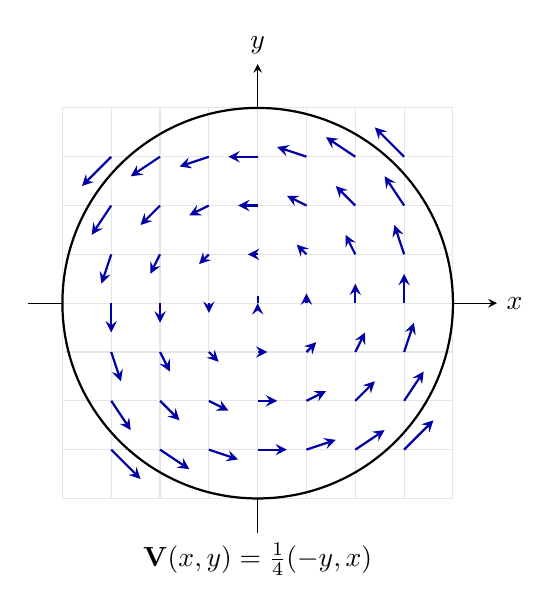
\begin{tikzpicture}[scale=0.62, >=stealth]
    \draw[->] (-4.7,0) -- (4.9,0) node[right] {\(x\)};
    \draw[->] (0,-4.7) -- (0,4.9) node[above] {\(y\)};

    \draw[gray!20, step=1] (-4,-4) grid (4,4);

    \foreach \x in {-3,-2,-1,0,1,2,3} {
        \foreach \y in {-3,-2,-1,0,1,2,3} {
            \draw[->, blue!65!black, thick]
                (\x,\y) -- ++({-0.20*\y},{0.20*\x});
        }
    }

    \draw[thick] (0,0) circle (4);
    \node at (0,-5.25) {\(\mathbf V(x,y)=\frac14(-y,x)\)};
\end{tikzpicture}
\caption{A vector field attaches an arrow to every point of its domain.}
\end{figure}

This picture is not one moving particle.  It is a whole instruction book.  If a tiny
floating leaf reaches the point \((2,3)\), the field tells the leaf what velocity to have
there:
\[
    \mathbf V(2,3)=\frac14(-3,2)=\left(-\frac34,\frac12\right).
\]

\begin{definition}[Vector field]
A \emph{vector field} on a region \(D\) in the plane is a function
\[
    \mathbf F:D\subseteq\mathbb R^2\to\mathbb R^2.
\]
Usually we write
\[
    \mathbf F(x,y)=(P(x,y),Q(x,y)).
\]

A vector field on a region \(D\) in space is a function
\[
    \mathbf F:D\subseteq\mathbb R^3\to\mathbb R^3,
\]
usually written
\[
    \mathbf F(x,y,z)=(P(x,y,z),Q(x,y,z),R(x,y,z)).
\]
\end{definition}

The input is a point.  The output is a vector.  We draw the output vector with its tail
placed at the input point.

The domain matters.  The formula
\[
    \mathbf F(x,y)=\frac{1}{x^2+y^2}(-y,x)
\]
looks like a swirling field, but it is not defined at the origin.  Its domain is
\[
    \mathbb R^2\setminus\{(0,0)\}.
\]
That missing point will become important later, when we study conservative fields.
A tiny hole can change the behavior of every closed curve around it.

\subsection{Velocity fields, force fields, and gradient fields}

Vector fields appear in several different roles.

A \emph{velocity field} tells how a fluid or moving crowd flows.  The fountain field
\[
    \mathbf V(x,y)=\frac14(-y,x)
\]
is a velocity field.  It assigns a velocity vector to every point in the water.

A \emph{force field} tells what force would act on a particle placed at each point.
For example, a simplified gravitational field pointing toward the origin has the form
\[
    \mathbf G(x,y,z)
    =
    -\frac{k}{(x^2+y^2+z^2)^{3/2}}(x,y,z),
\]
where \(k>0\).  The vector \((x,y,z)\) points away from the origin, so the negative sign
points back toward the origin.  The denominator says the field weakens with distance.

A \emph{gradient field} comes from a scalar field.  If
\[
    f(x,y)
\]
is a differentiable scalar field, then
\[
    \nabla f(x,y)=\bigl(f_x(x,y),f_y(x,y)\bigr)
\]
is a vector field.

For example, let
\[
    h(x,y)=100+4x+3y-x^2-y^2.
\]
This could be a simple height model for a hill.  Its gradient field is
\[
    \nabla h(x,y)=(4-2x,\;3-2y).
\]
At the point \((1,1)\),
\[
    \nabla h(1,1)=(2,1).
\]
A hiker standing there sees the steepest uphill direction pointing roughly east and
slightly north.

Recall from Section \ref{sec:9.1} that gradients cross level curves at right angles.
So a gradient field is not just a collection of arrows; it is tied to the contour map of
the scalar field that produced it.

\begin{example}[A field that is not a gradient field, at least not obviously]
The swirling field
\[
    \mathbf V(x,y)=(-y,x)
\]
has arrows tangent to circles centered at the origin.  If it were the gradient of some
height function, its arrows would be perpendicular to that height function's level
curves.  But these arrows go around in circles.  They look more like rotation than
uphill motion.

Later we will learn a test that detects this difference.  Some fields are gradients in
disguise.  Others carry genuine circulation.
\end{example}

\subsection{Sketching vector fields}

A vector field drawing cannot show every arrow.  There are infinitely many points.
A sketch chooses representative points and draws enough arrows to reveal the pattern.

Here are four basic fields in the plane.

\[
\begin{array}{c|c|c}
\text{Field} & \text{Formula} & \text{Pattern} \\ \hline
\text{constant field} & (1,0) & \text{all arrows point right}\\[1mm]
\text{radial source} & (x,y) & \text{arrows point away from the origin}\\[1mm]
\text{radial sink} & (-x,-y) & \text{arrows point toward the origin}\\[1mm]
\text{rotational field} & (-y,x) & \text{arrows circulate counterclockwise}
\end{array}
\]

The length of an arrow matters, but only up to the scale of the drawing.  If one arrow
is too long, it can hide the rest of the picture.  It is common to shorten all arrows
while preserving their directions, or to draw only direction arrows.  A sketch is meant
to show structure, not to be a measuring device.

\begin{example}[Sketching a saddle-like field]
Consider
\[
    \mathbf F(x,y)=(x,-y).
\]
On the \(x\)-axis, where \(y=0\),
\[
    \mathbf F(x,0)=(x,0).
\]
So arrows point away from the origin along the \(x\)-axis.

On the \(y\)-axis, where \(x=0\),
\[
    \mathbf F(0,y)=(0,-y).
\]
So arrows point toward the origin along the \(y\)-axis.

This field pushes outward in one direction and inward in the perpendicular direction.
The origin is a saddle-type equilibrium: motion near it is attracted from some
directions and repelled in others.
\end{example}

A few practical rules help when drawing a field.

\[
\begin{array}{c|l}
\text{Step} & \text{What to look for} \\ \hline
1 & \text{Evaluate the field at simple points.}\\
2 & \text{Look along axes or symmetry lines.}\\
3 & \text{Find points where }\mathbf F=\mathbf 0.\\
4 & \text{Notice whether arrows point outward, inward, around, or across.}\\
5 & \text{Scale arrows so the pattern can be seen.}
\end{array}
\]

The points where
\[
    \mathbf F(\mathbf p)=\mathbf 0
\]
are called \emph{equilibrium points}.  If the field is a velocity field, a particle placed
exactly at such a point does not move.

\subsection{Flow lines and qualitative behavior}

A vector field tells a moving particle what velocity it should have at each point.
A path that obeys the field is called a flow line.

For the fountain field
\[
    \mathbf V(x,y)=(-y,x),
\]
the circle
\[
    \mathbf r(t)=(R\cos t,R\sin t)
\]
is a flow line.  Its velocity is
\[
    \mathbf r'(t)=(-R\sin t,R\cos t).
\]
But
\[
    \mathbf V(\mathbf r(t))
    =
    \mathbf V(R\cos t,R\sin t)
    =
    (-R\sin t,R\cos t).
\]
So
\[
    \mathbf r'(t)=\mathbf V(\mathbf r(t)).
\]
The particle follows the arrows exactly.

\begin{definition}[Flow line]
Let \(\mathbf F\) be a vector field.  A differentiable curve
\[
    \mathbf r(t)
\]
is called a \emph{flow line} of \(\mathbf F\) if
\[
\boxed{
    \mathbf r'(t)=\mathbf F(\mathbf r(t))
}
\]
for every \(t\) in its interval of definition.
\end{definition}

The equation
\[
    \mathbf r'(t)=\mathbf F(\mathbf r(t))
\]
says that the curve's velocity at each moment equals the arrow assigned by the field
at the curve's current position.

\begin{example}[Flow lines of a radial field]
Let
\[
    \mathbf F(x,y)=(x,y).
\]
If a particle starts at
\[
    \mathbf r(0)=(a,b),
\]
then
\[
    \mathbf r(t)=(ae^t,be^t)
\]
is a flow line, because
\[
    \mathbf r'(t)=(ae^t,be^t)=\mathbf r(t)=\mathbf F(\mathbf r(t)).
\]
The particle moves along the ray through \((a,b)\), away from the origin.  The origin
is an equilibrium point, but nearby points are pushed outward.
\end{example}

\begin{example}[Flow lines of a saddle field]
For
\[
    \mathbf F(x,y)=(x,-y),
\]
a flow line through \((a,b)\) is
\[
    \mathbf r(t)=(ae^t,be^{-t}).
\]
Then
\[
    \mathbf r'(t)=(ae^t,-be^{-t})
    =
    \mathbf F(ae^t,be^{-t}).
\]
If \(ab\ne0\), the product of the coordinates along the flow is
\[
    x(t)y(t)=ae^t\cdot be^{-t}=ab.
\]
So the flow lines lie on hyperbolas
\[
    xy=\text{constant}.
\]
\end{example}

A vector field drawing is therefore a prediction device.  It tells us where motion is
fast or slow, where it turns, where it settles, and where it circulates.

But motion is only one thing we can do with a curve.  A curve can also carry material.
A wire can have density.  A trail can have snow depth.  A cable can have temperature.
Those quantities are not arrows, but they still need to be added along a path.  Before
we let vector fields do work, we need the simpler integral that adds scalar quantities
along curves.

\section{Line integrals of scalar functions}
\label{sec:13.2}

A vector field attaches arrows to points.  A scalar field attaches numbers.  When a
curve passes through a scalar field, it collects numbers along its length.

That idea sounds like ordinary integration, but the domain is no longer an interval.
The domain is a curve.

\subsection{Accumulating density along a curve}

A thin copper wire is bent into the upper half of a circle of radius \(3\).  Its shape is
\[
    x^2+y^2=9,
    \qquad
    y\ge0.
\]
The wire is not uniform.  Its linear density at the point \((x,y)\) is
\[
    \rho(x,y)=2+\frac{x}{3}
\]
grams per centimeter.

The right side of the wire is denser, because \(x>0\).  The left side is lighter, because
\(x<0\).

Parametrize the upper semicircle by
\[
    \mathbf r(t)=(3\cos t,3\sin t),
    \qquad
    0\le t\le \pi.
\]
Then
\[
    \rho(\mathbf r(t))
    =
    2+\frac{3\cos t}{3}
    =
    2+\cos t.
\]

A small change \(dt\) sweeps out a small arc length.  Since
\[
    \mathbf r'(t)=(-3\sin t,3\cos t),
\]
we have
\[
    \|\mathbf r'(t)\|
    =
    \sqrt{9\sin^2t+9\cos^2t}
    =
    3.
\]
So
\[
    ds=3\,dt.
\]
A small piece of wire has mass approximately
\[
    \rho(\mathbf r(t))\,ds
    =
    (2+\cos t)3\,dt.
\]
Adding all pieces gives
\[
\begin{aligned}
M
&=
\int_0^\pi (2+\cos t)3\,dt\\
&=
3\left[2t+\sin t\right]_0^\pi\\
&=
6\pi.
\end{aligned}
\]
So the wire has mass
\[
\boxed{
    6\pi \text{ grams}.
}
\]

\begin{figure}[h]
\centering
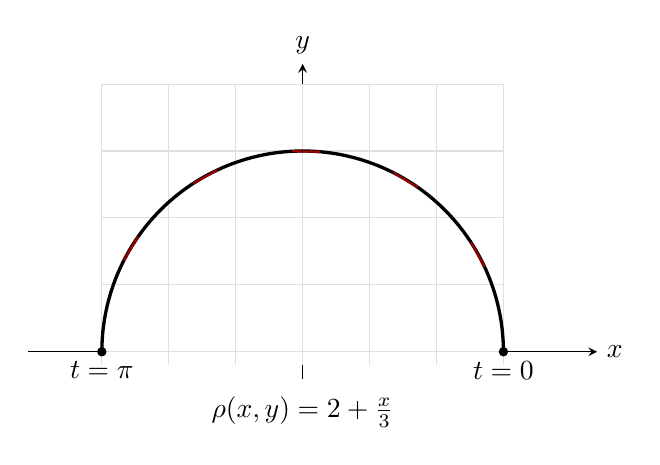
\begin{tikzpicture}[scale=0.85, >=stealth]
    \draw[->] (-4.1,0) -- (4.4,0) node[right] {\(x\)};
    \draw[->] (0,-0.4) -- (0,4.3) node[above] {\(y\)};

    \draw[gray!25, step=1] (-3,-0.2) grid (3,4);

    \draw[very thick, domain=0:180, samples=120, variable=\t]
        plot ({3*cos(\t)}, {3*sin(\t)});

    \foreach \a in {25,55,85,115,145} {
        \draw[red!60!black, thick]
            ({3*cos(\a)},{3*sin(\a)})
            -- ({3*cos(\a+8)},{3*sin(\a+8)});
    }

    \fill (3,0) circle (2pt);
    \fill (-3,0) circle (2pt);

    \node[below] at (3,0) {\(t=0\)};
    \node[below] at (-3,0) {\(t=\pi\)};
    \node at (0,-0.9) {\(\rho(x,y)=2+\frac{x}{3}\)};
\end{tikzpicture}
\caption{A scalar line integral adds density along the length of a curve.}
\end{figure}

This is the seed of the definition.  We multiply the scalar value on the curve by a tiny
length element and add:
\[
    \sum \rho\,\Delta s.
\]

\subsection{The arc length element \texorpdfstring{\(ds\)}{ds}}

The symbol
\[
    ds
\]
means a tiny piece of arc length.

If a curve is parametrized by
\[
    \mathbf r(t)=(x(t),y(t)),
\]
then over a small time interval \(\Delta t\), the displacement is approximately
\[
    \mathbf r'(t)\Delta t.
\]
Its length is approximately
\[
    \|\mathbf r'(t)\|\Delta t.
\]
So
\[
\boxed{
    ds=\|\mathbf r'(t)\|\,dt.
}
\]
In the plane,
\[
\boxed{
    ds=
    \sqrt{\left(\frac{dx}{dt}\right)^2+
          \left(\frac{dy}{dt}\right)^2}\,dt.
}
\]
In space,
\[
\boxed{
    ds=
    \sqrt{\left(\frac{dx}{dt}\right)^2+
          \left(\frac{dy}{dt}\right)^2+
          \left(\frac{dz}{dt}\right)^2}\,dt.
}
\]

This is the same speed from Chapter \ref{ch:5}.  Arc length is distance traveled:
\[
    L=\int_a^b \|\mathbf r'(t)\|\,dt.
\]
A scalar line integral simply weights this distance by a scalar field.

\begin{definition}[Line integral of a scalar function]
Let \(C\) be a piecewise smooth curve parametrized by
\[
    \mathbf r(t),\qquad a\le t\le b.
\]
Let \(f\) be a continuous scalar function on \(C\).  The \emph{line integral of \(f\)
with respect to arc length} is
\[
\boxed{
    \int_C f\,ds
    =
    \int_a^b f(\mathbf r(t))\,\|\mathbf r'(t)\|\,dt.
}
\]
\end{definition}

The notation
\[
    \int_C f\,ds
\]
says: add the values of \(f\) along the curve, weighted by length.

If
\[
    f=1,
\]
then
\[
    \int_C 1\,ds
    =
    \int_a^b \|\mathbf r'(t)\|\,dt,
\]
which is the length of the curve.

\subsection{Mass of a wire}

A scalar line integral is often a mass integral.

\begin{example}[A straight wire in space]
A wire runs from
\[
    (0,0,0)
\]
to
\[
    (2,2,1).
\]
Parametrize it by
\[
    \mathbf r(t)=(t,t,t/2),
    \qquad
    0\le t\le2.
\]
Suppose its density is
\[
    \rho(x,y,z)=1+z
\]
kilograms per meter.

Along the wire,
\[
    \rho(\mathbf r(t))=1+\frac t2.
\]
Also,
\[
    \mathbf r'(t)=\left(1,1,\frac12\right),
\]
so
\[
    \|\mathbf r'(t)\|
    =
    \sqrt{1+1+\frac14}
    =
    \frac32.
\]
Therefore
\[
\begin{aligned}
M
&=
\int_C \rho\,ds\\
&=
\int_0^2
\left(1+\frac t2\right)\frac32\,dt\\
&=
\frac32\left[t+\frac{t^2}{4}\right]_0^2\\
&=
\frac32(2+1)\\
&=
\frac92.
\end{aligned}
\]
So the wire has mass
\[
\boxed{
    \frac92 \text{ kilograms}.
}
\]
\end{example}

The computation has three steps:

\[
\begin{array}{c|c}
\text{Step} & \text{Action} \\ \hline
1 & \text{Parametrize the curve: }\mathbf r(t).\\[1mm]
2 & \text{Evaluate the scalar field on the curve: }f(\mathbf r(t)).\\[1mm]
3 & \text{Multiply by speed: }\|\mathbf r'(t)\|\,dt.
\end{array}
\]

The last step is the one students most often forget.  The parameter \(t\) is not
necessarily arc length.  The factor
\[
    \|\mathbf r'(t)\|
\]
converts \(dt\) into length.

\begin{example}[The same segment with a different clock]
The same line segment from \((0,0,0)\) to \((2,2,1)\) can also be written as
\[
    \mathbf q(u)=(2u,2u,u),
    \qquad
    0\le u\le1.
\]
Along this parametrization,
\[
    \rho(\mathbf q(u))=1+u,
\]
and
\[
    \mathbf q'(u)=(2,2,1),
\]
so
\[
    \|\mathbf q'(u)\|=3.
\]
The mass is
\[
\begin{aligned}
M
&=
\int_0^1 (1+u)3\,du\\
&=
3\left[u+\frac{u^2}{2}\right]_0^1\\
&=
\frac92.
\end{aligned}
\]
The answer is the same.  The new clock moves along the same wire over a different
parameter interval, and the speed factor corrects for that.
\end{example}

\subsection{Why parametrization does not change the value}

The last example was not an accident.  A scalar line integral depends on the curve as a
traced geometric object, not on the particular clock used to trace it.

\begin{theorem}[Scalar line integrals are unchanged by reparametrization]
Let \(C\) be a curve parametrized by
\[
    \mathbf r(t),\qquad a\le t\le b.
\]
Let
\[
    t=\phi(u),\qquad \alpha\le u\le \beta,
\]
where \(\phi\) is continuously differentiable and traces the interval \([a,b]\) exactly
once, either forward or backward.  Then
\[
    \mathbf q(u)=\mathbf r(\phi(u))
\]
parametrizes the same curve once, and
\[
\boxed{
    \int_\alpha^\beta
    f(\mathbf q(u))\|\mathbf q'(u)\|\,du
    =
    \int_a^b
    f(\mathbf r(t))\|\mathbf r'(t)\|\,dt.
}
\]
\end{theorem}

\begin{proof}
By the chain rule,
\[
    \mathbf q'(u)=\mathbf r'(\phi(u))\phi'(u).
\]
Therefore
\[
    \|\mathbf q'(u)\|
    =
    \|\mathbf r'(\phi(u))\|\,|\phi'(u)|.
\]
So
\[
    f(\mathbf q(u))\|\mathbf q'(u)\|
    =
    f(\mathbf r(\phi(u)))\|\mathbf r'(\phi(u))\|\,|\phi'(u)|.
\]
If \(\phi\) traces the interval forward, then \(\phi'(u)\ge0\) except possibly at isolated
points, and this is the ordinary substitution rule.  If \(\phi\) traces the interval
backward, the absolute value reverses the sign that would have come from \(dt\).
Either way, length is positive, and the same total is obtained.
\end{proof}

This is why orientation does not affect scalar line integrals.  If you walk along a wire
from left to right or right to left, its mass is the same.

But the theorem contains the phrase ``exactly once'' for a reason.

\begin{example}[Same image, different multiplicity]
Let \(C\) be the unit circle and let
\[
    f(x,y)=1.
\]
Tracing the circle once by
\[
    \mathbf r(t)=(\cos t,\sin t),
    \qquad 0\le t\le2\pi,
\]
gives
\[
    \int_C 1\,ds
    =
    \int_0^{2\pi}1\,dt
    =
    2\pi.
\]

Tracing the same geometric circle twice by
\[
    \mathbf q(t)=(\cos t,\sin t),
    \qquad 0\le t\le4\pi,
\]
gives
\[
    \int 1\,ds
    =
    \int_0^{4\pi}1\,dt
    =
    4\pi.
\]
The image is the same set of points, but the traced curve is not the same.  The second
parametrization counts the wire twice.
\end{example}

The phrase ``piecewise smooth'' also matters.  It rules out curves whose length is not
controlled by ordinary calculus.

\begin{example}[A continuous curve can have too much length]
Define
\[
    \mathbf r(t)=
    \begin{cases}
    (t,\;t\sin(1/t)), & 0<t\le1,\\
    (0,0), & t=0.
    \end{cases}
\]
This curve is continuous, but it wiggles infinitely often near the origin.  Its length is
infinite.  Therefore
\[
    \int_C 1\,ds
\]
does not give a finite number.

So continuity alone is not enough for the line integrals in this chapter.  Piecewise
smooth curves keep the geometry tame enough that arc length can be computed by
\[
    \int \|\mathbf r'(t)\|\,dt.
\]
\end{example}

The scalar field also needs to be reasonable along the curve.

\begin{example}[A density too wild to integrate]
On the line segment
\[
    \mathbf r(t)=(t,0),
    \qquad 0\le t\le1,
\]
define
\[
    f(x,y)=
    \begin{cases}
    1, & x \text{ rational},\\
    0, & x \text{ irrational}.
    \end{cases}
\]
Every subinterval contains rational and irrational \(x\)-values.  Riemann sums can be
forced toward \(1\) or toward \(0\), depending on sample points.  There is no single
settled value.

This is why the definition assumes \(f\) is continuous on the curve.  Continuous
densities do not jump between two values at every scale.
\end{example}

\subsection{Average value along a curve}

For a scalar function on a region, average value means
\[
    \frac{\text{total}}{\text{size of domain}}.
\]
Along a curve, the size of the domain is length.

\begin{definition}[Average value along a curve]
Let \(C\) have length
\[
    L=\int_C 1\,ds.
\]
The average value of a scalar function \(f\) along \(C\) is
\[
\boxed{
    f_{\mathrm{avg}}
    =
    \frac{1}{L}\int_C f\,ds.
}
\]
\end{definition}

\begin{example}[Average density on the semicircular wire]
For the upper semicircle of radius \(3\),
\[
    L=3\pi.
\]
Earlier we found
\[
    \int_C \rho\,ds=6\pi.
\]
Therefore the average density is
\[
    \rho_{\mathrm{avg}}
    =
    \frac{1}{3\pi}(6\pi)
    =
    2.
\]
This makes sense.  The density
\[
    \rho(x,y)=2+\frac{x}{3}
\]
is larger on the right side and smaller on the left side.  The upper semicircle is
symmetric, so the \(x/3\) part averages to \(0\).
\end{example}

\begin{example}[Average temperature along a straight cable]
A cable runs from
\[
    (0,0)
\]
to
\[
    (4,3).
\]
The temperature on the floor is
\[
    T(x,y)=18+x-\frac{y}{3}.
\]
Parametrize the cable by
\[
    \mathbf r(t)=(4t,3t),
    \qquad 0\le t\le1.
\]
Then
\[
    T(\mathbf r(t))
    =
    18+4t-\frac{3t}{3}
    =
    18+3t.
\]
Also,
\[
    \|\mathbf r'(t)\|=\|(4,3)\|=5.
\]
The length is
\[
    L=\int_0^1 5\,dt=5.
\]
The average temperature is
\[
\begin{aligned}
T_{\mathrm{avg}}
&=
\frac{1}{5}\int_0^1 (18+3t)5\,dt\\
&=
\int_0^1(18+3t)\,dt\\
&=
18+\frac32\\
&=
\frac{39}{2}.
\end{aligned}
\]
So the average temperature along the cable is
\[
\boxed{
    19.5^\circ\text{C}.
}
\]
\end{example}

Scalar line integrals add quantities that do not care which way the curve is traveled.
Mass, length, and average temperature are unchanged if we reverse direction.

A force field is different.  If a force helps you move one way, it resists you in the
opposite direction.  To measure work, we cannot multiply by the unsigned length
\(ds\).  We must measure how much of the force points along the actual displacement.
That is where
\[
    \mathbf F\cdot d\mathbf r
\]
enters, and it will lead us directly to the \(1\)-form
\[
    P\,dx+Q\,dy+R\,dz.
\]
\section{Work integrals of vector fields}
\label{sec:13.3}

Section \ref{sec:13.2} added scalar quantities along a curve.  Density, temperature,
and length used
\[
    ds,
\]
so direction did not matter.  Walking along a wire from left to right or right to left
does not change its mass.

Force is different.  A force that helps you move one way resists you in the opposite
way.  So a work integral cannot use only the unsigned length \(ds\).  It must remember
the actual displacement.

\subsection{Force dotted with displacement}

Start with a constant force.  A cart is pulled across a warehouse floor by the force
\[
    \mathbf F=(4,1)
\]
newtons.  The cart moves from
\[
    A=(0,0)
\]
to
\[
    B=(3,2).
\]
Its displacement is
\[
    \Delta \mathbf r=B-A=(3,2).
\]
The work done by the force is
\[
\begin{aligned}
W
&=
\mathbf F\cdot \Delta \mathbf r\\
&=
(4,1)\cdot(3,2)\\
&=
12+2\\
&=
14.
\end{aligned}
\]
The force has a large eastward component and a small northward component.  Both help
this displacement.

If the same cart moves backward from \(B\) to \(A\), the displacement is
\[
    -\Delta \mathbf r=(-3,-2).
\]
The work becomes
\[
    \mathbf F\cdot(-\Delta \mathbf r)=-14.
\]
The same force now resists the motion.

This is the first difference between scalar line integrals and work integrals:

\[
\boxed{
    \text{Scalar line integrals ignore orientation.  Work integrals remember it.}
}
\]

Now let the force vary from point to point, and let the cart move along a curved track.

Suppose the force field is
\[
    \mathbf F(x,y)=(2x,1).
\]
The eastward force grows as \(x\) increases, and the northward force is constantly \(1\).

Let the track be
\[
    \mathbf r(t)=(t,t^2),
    \qquad
    0\le t\le2.
\]
A tiny time step \(dt\) produces the tiny displacement
\[
    d\mathbf r\approx \mathbf r'(t)\,dt.
\]
Since
\[
    \mathbf r'(t)=(1,2t),
\]
and
\[
    \mathbf F(\mathbf r(t))=\mathbf F(t,t^2)=(2t,1),
\]
the tiny work is approximately
\[
\begin{aligned}
dW
&=
\mathbf F(\mathbf r(t))\cdot \mathbf r'(t)\,dt\\
&=
(2t,1)\cdot(1,2t)\,dt\\
&=
(2t+2t)\,dt\\
&=
4t\,dt.
\end{aligned}
\]
Adding all the tiny work pieces gives
\[
\begin{aligned}
W
&=
\int_0^2 4t\,dt\\
&=
\left[2t^2\right]_0^2\\
&=
8.
\end{aligned}
\]

\begin{figure}[h]
\centering
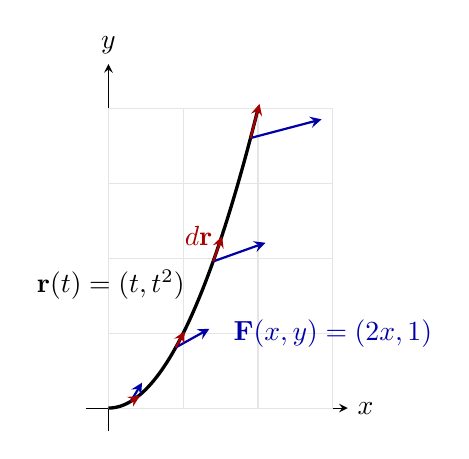
\begin{tikzpicture}[scale=0.95, >=stealth]
    \draw[->] (-0.3,0) -- (3.2,0) node[right] {\(x\)};
    \draw[->] (0,-0.3) -- (0,4.6) node[above] {\(y\)};

    \draw[gray!20, step=1] (0,0) grid (3,4);

    \draw[very thick, domain=0:2, samples=100, variable=\t]
        plot ({\t},{\t*\t});

    % Floating label for the curve, placed cleanly to its upper-left
    \node[above left] at (1.15,1.3225) {\(\mathbf r(t)=(t,t^2)\)};

    % Calculates the y-coordinate mathematically to guarantee it sits on the curve
    \foreach \x in {0.3, 0.9, 1.4, 1.9} {
        % Force vector F (blue)
        \draw[->, blue!65!black, thick]
            (\x,{\x*\x}) -- ++({0.25*(2*\x)},{0.25});
            
        % Tiny displacement vector dr (red, strictly tangent to the curve)
        \draw[->, red!65!black, thick]
            (\x,{\x*\x}) -- ++(0.12,{0.12*2*\x});
    }

    % Label one of the dr vectors (e.g., the one at x=1.4) to define them
    \node[red!65!black, left] at ({1.4+0.12},{1.4*1.4+0.12*2*1.4}) {\(d\mathbf{r}\)};

    \node[blue!65!black] at (3.0,1.0) {\(\mathbf F(x,y)=(2x,1)\)};
\end{tikzpicture}
\caption{Work adds the component of the force in the direction of motion.}
\end{figure}

The dot product is doing the physical filtering.  Only the part of the force pointing
along the displacement contributes positive work.  The part perpendicular to the motion
does no work.

\subsection{\texorpdfstring{\(\int_C \mathbf F\cdot d\mathbf r\)}{integral F dot dr}}

The previous computation is the model for the definition.

Let
\[
    \mathbf F(x,y)=(P(x,y),Q(x,y))
\]
be a vector field in the plane, and let
\[
    \mathbf r(t)=(x(t),y(t)),
    \qquad
    a\le t\le b,
\]
parametrize an oriented curve \(C\).  Then
\[
    \mathbf r'(t)=(x'(t),y'(t)).
\]
The force at the point \(\mathbf r(t)\) is
\[
    \mathbf F(\mathbf r(t)).
\]
The tiny displacement is
\[
    d\mathbf r=\mathbf r'(t)\,dt.
\]
So the tiny work is
\[
    \mathbf F(\mathbf r(t))\cdot \mathbf r'(t)\,dt.
\]

\begin{definition}[Work integral of a vector field]
Let \(C\) be a piecewise smooth oriented curve parametrized by
\[
    \mathbf r(t),
    \qquad
    a\le t\le b.
\]
Let \(\mathbf F\) be a continuous vector field on \(C\).  The \emph{work integral} of
\(\mathbf F\) along \(C\) is
\[
\boxed{
    \int_C \mathbf F\cdot d\mathbf r
    =
    \int_a^b \mathbf F(\mathbf r(t))\cdot \mathbf r'(t)\,dt.
}
\]
\end{definition}

In the plane, this means
\[
\boxed{
    \int_C \mathbf F\cdot d\mathbf r
    =
    \int_a^b
    \left[
        P(x(t),y(t))x'(t)
        +
        Q(x(t),y(t))y'(t)
    \right]dt.
}
\]

In space, if
\[
    \mathbf F(x,y,z)=(P(x,y,z),Q(x,y,z),R(x,y,z))
\]
and
\[
    \mathbf r(t)=(x(t),y(t),z(t)),
\]
then
\[
\boxed{
    \int_C \mathbf F\cdot d\mathbf r
    =
    \int_a^b
    \left[
        P x'(t)+Q y'(t)+R z'(t)
    \right]dt,
}
\]
where \(P,Q,R\) are evaluated at
\[
    (x(t),y(t),z(t)).
\]

The notation
\[
    d\mathbf r
\]
is a reminder of the tiny displacement.  Along a parametrized curve,
\[
    d\mathbf r=\mathbf r'(t)\,dt.
\]

\begin{example}[Work along a helix]
A particle moves along the helix
\[
    \mathbf r(t)=(\cos t,\sin t,t),
    \qquad
    0\le t\le2\pi.
\]
A force field is
\[
    \mathbf F(x,y,z)=(-y,x,2).
\]
Find the work done along the helix.

First,
\[
    \mathbf r'(t)=(-\sin t,\cos t,1).
\]
Along the curve,
\[
    \mathbf F(\mathbf r(t))
    =
    \mathbf F(\cos t,\sin t,t)
    =
    (-\sin t,\cos t,2).
\]
Therefore
\[
\begin{aligned}
\mathbf F(\mathbf r(t))\cdot\mathbf r'(t)
&=
(-\sin t,\cos t,2)\cdot(-\sin t,\cos t,1)\\
&=
\sin^2t+\cos^2t+2\\
&=
3.
\end{aligned}
\]
So
\[
\boxed{
    \int_C \mathbf F\cdot d\mathbf r
    =
    \int_0^{2\pi}3\,dt
    =
    6\pi.
}
\]
The rotational part of the force helps the circular motion, and the constant vertical
force helps the upward motion.
\end{example}

\subsection{Parametrization and orientation of a curve}

A scalar line integral used
\[
    ds=\|\mathbf r'(t)\|\,dt.
\]
The absolute value hidden in the norm erased direction.  Work integrals use
\[
    d\mathbf r=\mathbf r'(t)\,dt.
\]
No absolute value appears.  Direction survives.

Return to the curved track
\[
    \mathbf r(t)=(t,t^2),
    \qquad
    0\le t\le2,
\]
with force field
\[
    \mathbf F(x,y)=(2x,1).
\]
We found
\[
    \int_C \mathbf F\cdot d\mathbf r=8.
\]

Now use a different clock:
\[
    \mathbf q(u)=(2u,4u^2),
    \qquad
    0\le u\le1.
\]
This traces the same curve in the same direction.  Along this parametrization,
\[
    \mathbf q'(u)=(2,8u),
\]
and
\[
    \mathbf F(\mathbf q(u))=(4u,1).
\]
Therefore
\[
\begin{aligned}
\int_0^1 \mathbf F(\mathbf q(u))\cdot\mathbf q'(u)\,du
&=
\int_0^1 (4u,1)\cdot(2,8u)\,du\\
&=
\int_0^1 16u\,du\\
&=
8.
\end{aligned}
\]
The value did not change.

Now reverse the curve:
\[
    \overline{\mathbf r}(t)=\mathbf r(2-t)
    =
    (2-t,(2-t)^2),
    \qquad
    0\le t\le2.
\]
Then
\[
    \overline{\mathbf r}'(t)=(-1,-2(2-t)).
\]
Also,
\[
    \mathbf F(\overline{\mathbf r}(t))=(2(2-t),1).
\]
Thus
\[
\begin{aligned}
\int_0^2
\mathbf F(\overline{\mathbf r}(t))\cdot \overline{\mathbf r}'(t)\,dt
&=
\int_0^2
\left[
    -2(2-t)-2(2-t)
\right]dt\\
&=
\int_0^2 -4(2-t)\,dt\\
&=
-8.
\end{aligned}
\]
Reversing the path reversed the sign.

\begin{theorem}[Effect of reparametrization on work integrals]
Let
\[
    \mathbf r(t),\qquad a\le t\le b,
\]
parametrize a piecewise smooth curve \(C\), and let
\[
    \mathbf q(u)=\mathbf r(\phi(u)),
    \qquad
    \alpha\le u\le\beta,
\]
where \(\phi\) is differentiable and traces \([a,b]\) exactly once.

If \(\phi\) is increasing, then \(\mathbf q\) gives the same orientation and
\[
\boxed{
    \int_\alpha^\beta
    \mathbf F(\mathbf q(u))\cdot\mathbf q'(u)\,du
    =
    \int_a^b
    \mathbf F(\mathbf r(t))\cdot\mathbf r'(t)\,dt.
}
\]

If \(\phi\) is decreasing, then \(\mathbf q\) gives the opposite orientation and
\[
\boxed{
    \int_\alpha^\beta
    \mathbf F(\mathbf q(u))\cdot\mathbf q'(u)\,du
    =
    -
    \int_a^b
    \mathbf F(\mathbf r(t))\cdot\mathbf r'(t)\,dt.
}
\]
\end{theorem}

\begin{proof}
By the chain rule,
\[
    \mathbf q'(u)=\mathbf r'(\phi(u))\phi'(u).
\]
Therefore
\[
\begin{aligned}
\mathbf F(\mathbf q(u))\cdot\mathbf q'(u)
&=
\mathbf F(\mathbf r(\phi(u)))\cdot
\bigl(\mathbf r'(\phi(u))\phi'(u)\bigr)\\
&=
\left[
\mathbf F(\mathbf r(\phi(u)))\cdot
\mathbf r'(\phi(u))
\right]\phi'(u).
\end{aligned}
\]
If \(\phi\) is increasing, the substitution \(t=\phi(u)\) preserves the order of the
limits.  If \(\phi\) is decreasing, the substitution reverses the order of the limits, which
introduces the minus sign.
\end{proof}

The phrase ``exactly once'' matters.  If the same curve is traced twice, the work is
counted twice.

\begin{example}[Same image, different multiplicity]
Let
\[
    \mathbf F(x,y)=(-y,x)
\]
and trace the unit circle by
\[
    \mathbf r(t)=(\cos t,\sin t).
\]
For one counterclockwise trip,
\[
    0\le t\le2\pi,
\]
we have
\[
    \mathbf F(\mathbf r(t))=(-\sin t,\cos t)
\]
and
\[
    \mathbf r'(t)=(-\sin t,\cos t).
\]
Thus
\[
    \mathbf F(\mathbf r(t))\cdot\mathbf r'(t)=1,
\]
so
\[
    \int_C \mathbf F\cdot d\mathbf r
    =
    \int_0^{2\pi}1\,dt
    =
    2\pi.
\]

If the same formula is used on
\[
    0\le t\le4\pi,
\]
the image is still the unit circle, but it is traced twice.  The integral becomes
\[
    \int_0^{4\pi}1\,dt=4\pi.
\]
The work integral sees the traveled curve with its multiplicity, not just the set of
points.
\end{example}

The continuity assumption on the vector field is also there for a reason.

\begin{example}[Why the field should be integrable along the path]
On the line segment
\[
    \mathbf r(t)=(t,0),
    \qquad
    0\le t\le1,
\]
define
\[
    \mathbf F(x,y)=(D(x),0),
\]
where
\[
    D(x)=
    \begin{cases}
    1, & x \text{ rational},\\
    0, & x \text{ irrational}.
    \end{cases}
\]
Then
\[
    \mathbf F(\mathbf r(t))\cdot\mathbf r'(t)=D(t).
\]
This function has no Riemann integral on \([0,1]\), because every interval contains
rational and irrational numbers.  The work sums can be forced toward different values
by different sample points.

Continuity is more than a comfort condition.  It prevents this kind of microscopic
jumping along the curve.
\end{example}

The curve itself must also be tame enough to have a velocity on finitely many smooth
pieces.  Corners are allowed; infinitely wild motion is not part of the basic theory here.

\subsection{Circulation around a closed curve}

When the curve is closed, work has a special name.

\begin{definition}[Circulation]
If \(C\) is a closed oriented curve and \(\mathbf F\) is a vector field, then
\[
\boxed{
    \oint_C \mathbf F\cdot d\mathbf r
}
\]
is called the \emph{circulation} of \(\mathbf F\) around \(C\).
\end{definition}

The circle on the integral sign reminds us that the curve is closed.  In the plane, a
counterclockwise orientation is usually called positive.  As you walk, the region inside
the curve stays on your left.

\begin{example}[A swirling field has positive circulation]
Let
\[
    \mathbf F(x,y)=(-y,x).
\]
This field points tangent to circles centered at the origin.  Around the unit circle,
parametrized counterclockwise by
\[
    \mathbf r(t)=(\cos t,\sin t),
    \qquad
    0\le t\le2\pi,
\]
we already computed
\[
    \mathbf F(\mathbf r(t))\cdot\mathbf r'(t)=1.
\]
Therefore
\[
\boxed{
    \oint_C \mathbf F\cdot d\mathbf r=2\pi.
}
\]

The arrows of the field point with the motion all the way around the circle.
\end{example}

\begin{figure}[h]
\centering
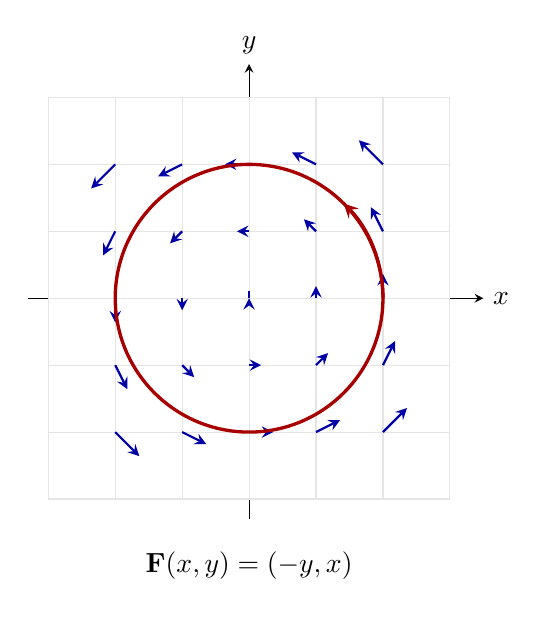
\begin{tikzpicture}[scale=0.85, >=stealth]
    \draw[->] (-3.3,0) -- (3.5,0) node[right] {\(x\)};
    \draw[->] (0,-3.3) -- (0,3.5) node[above] {\(y\)};

    \draw[gray!20, step=1] (-3,-3) grid (3,3);

    \foreach \x in {-2,-1,0,1,2} {
        \foreach \y in {-2,-1,0,1,2} {
            \draw[->, blue!65!black, thick]
                (\x,\y) -- ++({-0.18*\y},{0.18*\x});
        }
    }

    \draw[very thick, red!65!black] (0,0) circle (2);
    \draw[->, very thick, red!65!black] (2,0) arc[start angle=0,end angle=45,radius=2];

    \node at (0,-4.0) {\(\mathbf F(x,y)=(-y,x)\)};
\end{tikzpicture}
\caption{The field \((-y,x)\) circulates counterclockwise around the origin.}
\end{figure}

\begin{example}[A radial field has zero circulation around a circle]
Let
\[
    \mathbf G(x,y)=(x,y).
\]
On the unit circle,
\[
    \mathbf r(t)=(\cos t,\sin t),
\]
so
\[
    \mathbf G(\mathbf r(t))=(\cos t,\sin t).
\]
But
\[
    \mathbf r'(t)=(-\sin t,\cos t).
\]
Thus
\[
\begin{aligned}
\mathbf G(\mathbf r(t))\cdot\mathbf r'(t)
&=
(\cos t,\sin t)\cdot(-\sin t,\cos t)\\
&=
-\sin t\cos t+\sin t\cos t\\
&=
0.
\end{aligned}
\]
So
\[
\boxed{
    \oint_C \mathbf G\cdot d\mathbf r=0.
}
\]

The radial field points outward.  The circular motion is tangent.  A perpendicular force
does no work along the curve.
\end{example}

The two fields
\[
    (-y,x)
    \qquad\text{and}\qquad
    (x,y)
\]
look equally simple, but their closed-curve behavior is completely different.  One
carries circulation.  The other does not.

The dot-product notation
\[
    \mathbf F\cdot d\mathbf r
\]
has brought us far enough to compute work.  But it is hiding the actual integrand.
When
\[
    \mathbf F=(P,Q,R)
\]
and
\[
    d\mathbf r=(dx,dy,dz),
\]
the expression is really
\[
    P\,dx+Q\,dy+R\,dz.
\]
That object is not quite a vector field.  It is a \(1\)-form, and it is built from the
start to be integrated along a curve.

\section{Differential 1-forms}
\label{sec:13.4}

Section \ref{sec:13.3} defined work by
\[
    \int_C \mathbf F\cdot d\mathbf r.
\]
If
\[
    \mathbf F=(P,Q,R)
\]
and
\[
    \mathbf r(t)=(x(t),y(t),z(t)),
\]
then the integrand is
\[
    P x'(t)+Q y'(t)+R z'(t).
\]
But
\[
    x'(t)\,dt=dx,\qquad y'(t)\,dt=dy,\qquad z'(t)\,dt=dz.
\]
So the work integrand is really
\[
    P\,dx+Q\,dy+R\,dz.
\]

This is the point where differential forms enter the story as integrands, not as
abstract algebra.

\subsection{Work written as \texorpdfstring{\(P\,dx+Q\,dy+R\,dz\)}{P dx + Q dy + R dz}}

Return to the swirling field
\[
    \mathbf F(x,y)=(-y,x).
\]
The work expression is
\[
    \mathbf F\cdot d\mathbf r
    =
    (-y,x)\cdot(dx,dy)
    =
    -y\,dx+x\,dy.
\]
So instead of writing
\[
    \int_C \mathbf F\cdot d\mathbf r,
\]
we can write
\[
    \int_C -y\,dx+x\,dy.
\]

Let \(C\) be the unit circle oriented counterclockwise:
\[
    \mathbf r(t)=(\cos t,\sin t),
    \qquad
    0\le t\le2\pi.
\]
Along this curve,
\[
    x=\cos t,\qquad y=\sin t,
\]
so
\[
    dx=-\sin t\,dt,
    \qquad
    dy=\cos t\,dt.
\]
Substitute into the expression
\[
    -y\,dx+x\,dy:
\]
\[
\begin{aligned}
-y\,dx+x\,dy
&=
-(\sin t)(-\sin t\,dt)+(\cos t)(\cos t\,dt)\\
&=
(\sin^2 t+\cos^2 t)\,dt\\
&=
dt.
\end{aligned}
\]
Therefore
\[
\boxed{
    \int_C -y\,dx+x\,dy
    =
    \int_0^{2\pi}dt
    =
    2\pi.
}
\]

The calculation is the same as the work integral, but the notation has changed.  The
expression
\[
    -y\,dx+x\,dy
\]
is the object being integrated.  It knows how to eat tiny steps along a curve:
multiply the tiny \(x\)-step by \(-y\), multiply the tiny \(y\)-step by \(x\), and add.

\begin{definition}[Differential \(1\)-form]
A \emph{differential \(1\)-form} on a region \(D\) in the plane is an expression
\[
\boxed{
    \omega=P(x,y)\,dx+Q(x,y)\,dy.
}
\]
A differential \(1\)-form on a region \(D\) in space is an expression
\[
\boxed{
    \omega=P(x,y,z)\,dx+Q(x,y,z)\,dy+R(x,y,z)\,dz.
}
\]
The coefficient functions \(P,Q,R\) are scalar functions on \(D\).
\end{definition}

The symbols
\[
    dx,\qquad dy,\qquad dz
\]
are the coordinate-reading \(1\)-forms.  They measure components of a displacement:
\[
    dx(v_1,v_2,v_3)=v_1,
\]
\[
    dy(v_1,v_2,v_3)=v_2,
\]
and
\[
    dz(v_1,v_2,v_3)=v_3.
\]
So at a point \(\mathbf p\), the \(1\)-form
\[
    \omega=P\,dx+Q\,dy+R\,dz
\]
acts on a displacement vector
\[
    \mathbf v=(v_1,v_2,v_3)
\]
by
\[
\boxed{
    \omega_{\mathbf p}(\mathbf v)
    =
    P(\mathbf p)v_1+Q(\mathbf p)v_2+R(\mathbf p)v_3.
}
\]

A \(1\)-form is therefore a field of linear measuring rules.  At each point, it takes a
tiny displacement and returns a number.

\subsection{Why a \(1\)-form naturally integrates along a curve}

A curve supplies tiny displacements:
\[
    d\mathbf r=(dx,dy,dz).
\]
A \(1\)-form is built to measure those tiny displacements:
\[
    P\,dx+Q\,dy+R\,dz.
\]
That is why \(1\)-forms are the natural integrands along curves.

\begin{example}[A form along a parabolic track]
Let
\[
    \omega=y\,dx+x\,dy
\]
and let
\[
    \mathbf r(t)=(t,t^2),
    \qquad
    0\le t\le1.
\]
Then
\[
    x=t,\qquad y=t^2,
\]
so
\[
    dx=dt,
    \qquad
    dy=2t\,dt.
\]
Substitute:
\[
\begin{aligned}
\omega
&=
y\,dx+x\,dy\\
&=
t^2(dt)+t(2t\,dt)\\
&=
3t^2\,dt.
\end{aligned}
\]
Therefore
\[
\boxed{
    \int_C \omega
    =
    \int_0^1 3t^2\,dt
    =
    1.
}
\]

Something interesting happened here.  The answer is
\[
    1,
\]
which is also the change in
\[
    xy
\]
from the beginning of the curve to the end:
\[
    xy\big|_{(1,1)}-xy\big|_{(0,0)}=1-0=1.
\]
That is not a coincidence.  The next section will name the reason.
\end{example}

A \(1\)-form does not need a length element \(ds\).  It does not ask how long the
motion was.  It asks how much \(x\), \(y\), and \(z\) changed, with coefficients attached
to those changes.

That is why orientation matters.  Reverse a curve, and
\[
    dx,\ dy,\ dz
\]
all reverse sign.

\subsection{Pulling a \(1\)-form back to a parameter interval}

A curve turns a \(1\)-form into an ordinary single-variable integrand.

Let
\[
    \omega=P\,dx+Q\,dy+R\,dz
\]
and let
\[
    \mathbf r(t)=(x(t),y(t),z(t)),
    \qquad
    a\le t\le b.
\]
Along the curve,
\[
    dx=x'(t)\,dt,
    \qquad
    dy=y'(t)\,dt,
    \qquad
    dz=z'(t)\,dt.
\]
So
\[
\omega
\]
becomes
\[
\left[
P(\mathbf r(t))x'(t)
+
Q(\mathbf r(t))y'(t)
+
R(\mathbf r(t))z'(t)
\right]dt.
\]

\begin{definition}[Pullback of a \(1\)-form to a curve]
Let
\[
    \omega=P\,dx+Q\,dy+R\,dz
\]
be a \(1\)-form, and let
\[
    \mathbf r(t)=(x(t),y(t),z(t)).
\]
The \emph{pullback} of \(\omega\) by \(\mathbf r\) is the \(1\)-variable form
\[
\boxed{
    \mathbf r^*\omega
    =
    \left[
    P(\mathbf r(t))x'(t)
    +
    Q(\mathbf r(t))y'(t)
    +
    R(\mathbf r(t))z'(t)
    \right]dt.
}
\]
The line integral of \(\omega\) along \(C\) is
\[
\boxed{
    \int_C \omega
    =
    \int_a^b \mathbf r^*\omega.
}
\]
\end{definition}

The word \emph{pullback} means that the form has been pulled back from the curve in
space to the parameter interval on the \(t\)-line.  Once that happens, the integral is an
ordinary single-variable integral.

\begin{example}[Pulling back a space form]
Let
\[
    \omega=z\,dx+x\,dy+y\,dz.
\]
Let the curve be
\[
    \mathbf r(t)=(t,t^2,1-t),
    \qquad
    0\le t\le1.
\]
Then
\[
    dx=dt,
    \qquad
    dy=2t\,dt,
    \qquad
    dz=-dt.
\]
Also,
\[
    x=t,\qquad y=t^2,\qquad z=1-t.
\]
So
\[
\begin{aligned}
\mathbf r^*\omega
&=
(1-t)\,dt+t(2t\,dt)+t^2(-dt)\\
&=
(1-t+2t^2-t^2)\,dt\\
&=
(1-t+t^2)\,dt.
\end{aligned}
\]
Therefore
\[
\begin{aligned}
\int_C \omega
&=
\int_0^1(1-t+t^2)\,dt\\
&=
\left[t-\frac{t^2}{2}+\frac{t^3}{3}\right]_0^1\\
&=
1-\frac12+\frac13\\
&=
\frac56.
\end{aligned}
\]
\end{example}

The same hypotheses from work integrals remain.  The curve should be piecewise smooth,
and the coefficients of the form should be continuous along the curve.  Otherwise the
pulled-back integrand may not be integrable.

\begin{example}[A \(1\)-form too wild along a path]
Let
\[
    \omega=D(x)\,dx,
\]
where
\[
    D(x)=
    \begin{cases}
    1, & x \text{ rational},\\
    0, & x \text{ irrational}.
    \end{cases}
\]
Along the line segment
\[
    \mathbf r(t)=(t,0),
    \qquad
    0\le t\le1,
\]
we get
\[
    dx=dt,
\]
so
\[
    \mathbf r^*\omega=D(t)\,dt.
\]
This is not Riemann integrable.  The problem is not the curve.  The problem is that the
coefficient jumps between \(0\) and \(1\) at every scale.
\end{example}

Tracing a curve more than once also matters.

\begin{example}[The same image counted twice]
On the punctured plane
\[
    \mathbb R^2\setminus\{(0,0)\},
\]
consider the form
\[
    \omega=\frac{-y\,dx+x\,dy}{x^2+y^2}.
\]
On the unit circle
\[
    \mathbf r(t)=(\cos t,\sin t),
\]
we have
\[
    dx=-\sin t\,dt,
    \qquad
    dy=\cos t\,dt,
\]
so
\[
\begin{aligned}
\mathbf r^*\omega
&=
\frac{-(\sin t)(-\sin t\,dt)+(\cos t)(\cos t\,dt)}
{\cos^2t+\sin^2t}\\
&=
dt.
\end{aligned}
\]
One counterclockwise trip gives
\[
    \int_0^{2\pi}dt=2\pi.
\]
Two counterclockwise trips give
\[
    \int_0^{4\pi}dt=4\pi.
\]
The image is the same circle, but the traveled curve is different.
\end{example}

This form will return.  It measures change in angle.  It is locally called
\[
    d\theta,
\]
but the whole punctured plane has no single continuous angle function \(\theta\).  That
small fact is the source of a large surprise later.

\subsection{Vector fields and \(1\)-forms: related but not identical}

A vector field assigns an arrow to each point.  A \(1\)-form assigns a measuring rule to
each point.

In ordinary Cartesian coordinates, the dot product lets us turn a vector field into a
\(1\)-form.  If
\[
    \mathbf F=(P,Q,R),
\]
then the associated work form is
\[
\boxed{
    \omega_{\mathbf F}=P\,dx+Q\,dy+R\,dz.
}
\]
For every displacement vector \(\mathbf v\),
\[
    \omega_{\mathbf F}(\mathbf v)=\mathbf F\cdot\mathbf v.
\]
So
\[
\boxed{
    \int_C \mathbf F\cdot d\mathbf r
    =
    \int_C \omega_{\mathbf F}.
}
\]

That is why vector fields and \(1\)-forms look almost the same in this chapter.  But
they are not the same kind of object.

The distinction becomes visible in polar coordinates.

A small displacement in the plane can be written as
\[
    d\mathbf r=\mathbf e_r\,dr+\mathbf e_\theta\,r\,d\theta.
\]
The factor \(r\) appears because a small angular change \(d\theta\) at radius \(r\) sweeps
out an arc of length
\[
    r\,d\theta.
\]

If a vector field is written in polar unit vectors as
\[
    \mathbf F=F_r\,\mathbf e_r+F_\theta\,\mathbf e_\theta,
\]
then its work form is
\[
\boxed{
    \mathbf F\cdot d\mathbf r
    =
    F_r\,dr+F_\theta\,r\,d\theta.
}
\]
The angular part gets a factor of \(r\).

\begin{example}[The angular unit vector and the angle form]
The unit angular vector field is
\[
    \mathbf e_\theta=(-\sin\theta,\cos\theta)
    =
    \left(-\frac{y}{r},\frac{x}{r}\right),
\]
where
\[
    r=\sqrt{x^2+y^2}.
\]
Its associated work form is
\[
    \omega_{\mathbf e_\theta}
    =
    -\frac{y}{r}\,dx+\frac{x}{r}\,dy.
\]
Since
\[
    d\theta=
    \frac{-y\,dx+x\,dy}{r^2},
\]
we have
\[
\boxed{
    \omega_{\mathbf e_\theta}=r\,d\theta.
}
\]

On a circle of radius \(R\),
\[
    r\,d\theta=R\,d\theta.
\]
So
\[
    \int_{\text{circle}} \omega_{\mathbf e_\theta}
    =
    \int_0^{2\pi}R\,d\theta
    =
    2\pi R.
\]
That is the circumference.  A unit tangent force does one unit of work per unit of arc
length.

But the form
\[
    d\theta
\]
itself gives
\[
    \int_{\text{circle}}d\theta=2\pi.
\]
It measures angle swept out, not distance traveled.

The vector field corresponding to \(d\theta\) by the Cartesian dot product is
\[
    \left(-\frac{y}{r^2},\frac{x}{r^2}\right),
\]
whose length is
\[
    \frac1r.
\]
So \(d\theta\) is not the work form of the unit angular vector field.  It is the work form
of a field whose arrows get weaker as the radius grows.
\end{example}

This example is worth keeping.  The vector field
\[
    \mathbf e_\theta
\]
is an arrow field.  The form
\[
    d\theta
\]
is an angle-measuring rule.  In Cartesian coordinates, a dot product connects arrows
and measuring rules, but the connection uses the geometry of the plane.

For line integrals, the \(1\)-form is the cleaner object:
\[
    \int_C P\,dx+Q\,dy+R\,dz.
\]
It says exactly what is added along the curve.

Some \(1\)-forms have a special origin.  The form
\[
    y\,dx+x\,dy
\]
from the earlier example is
\[
    d(xy).
\]
It is the differential of a function.  That is why its integral along the parabola quietly
became an endpoint difference.

But the angle form
\[
    \frac{-y\,dx+x\,dy}{x^2+y^2}
\]
also looks like it should be \(d\theta\), and its integral around a closed circle is
\[
    2\pi,
\]
not \(0\).  How can a differential around a closed loop fail to cancel?

The answer depends not only on the formula, but on the domain.  A missing point can
change everything.  That is where conservative vector fields and exact \(1\)-forms
begin.
\section{Conservative vector fields and exact \(1\)-forms}
\label{sec:13.5}

Section \ref{sec:13.4} ended with a small mystery.  The form
\[
    y\,dx+x\,dy
\]
quietly became an endpoint difference, because
\[
    y\,dx+x\,dy=d(xy).
\]
But the angle form
\[
    \frac{-y\,dx+x\,dy}{x^2+y^2}
\]
looked like it wanted to be \(d\theta\), while its integral around a circle was not zero.
So the question is now unavoidable:

\[
    \text{When is a line integral really just an endpoint difference?}
\]

\subsection{Potential functions}

Start with a force field on a factory floor:
\[
    \mathbf F(x,y)=(y,x).
\]
Its work form is
\[
    \omega=\mathbf F\cdot d\mathbf r=y\,dx+x\,dy.
\]

Move a cart from
\[
    A=(0,0)
\]
to
\[
    B=(2,1).
\]
First take the straight path
\[
    \mathbf r(t)=(2t,t),
    \qquad 0\le t\le1.
\]
Along this path,
\[
    x=2t,\qquad y=t,
\]
so
\[
    dx=2\,dt,\qquad dy=dt.
\]
Therefore
\[
\begin{aligned}
\omega
&=
y\,dx+x\,dy\\
&=
t(2\,dt)+(2t)(dt)\\
&=
4t\,dt.
\end{aligned}
\]
The work is
\[
    \int_0^1 4t\,dt=2.
\]

Now take a broken path: first go east from \((0,0)\) to \((2,0)\), then go north from
\((2,0)\) to \((2,1)\).

On the eastward segment,
\[
    y=0,\qquad dy=0,
\]
so
\[
    y\,dx+x\,dy=0.
\]
On the northward segment,
\[
    x=2,\qquad dx=0,
\]
so
\[
    y\,dx+x\,dy=2\,dy.
\]
Thus
\[
    \int_0^1 2\,dy=2.
\]
Both paths give the same work.

\begin{figure}[h]
\centering
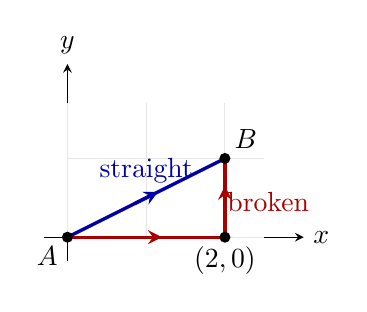
\begin{tikzpicture}[scale=1.0, >=stealth]
    \draw[->] (-0.3,0) -- (3.0,0) node[right] {\(x\)};
    \draw[->] (0,-0.3) -- (0,2.2) node[above] {\(y\)};

    \draw[gray!20, step=1] (0,0) grid (2.5,1.7);

    \coordinate (A) at (0,0);
    \coordinate (B) at (2,1);
    \coordinate (M) at (2,0);

    \draw[very thick, blue!65!black] (A) -- (B);
    \draw[->, very thick, blue!65!black] (0.85,0.425) -- (1.15,0.575);

    \draw[very thick, red!65!black] (A) -- (M) -- (B);
    \draw[->, very thick, red!65!black] (0.8,0) -- (1.2,0);
    \draw[->, very thick, red!65!black] (2,0.35) -- (2,0.65);

    \fill (A) circle (2pt);
    \fill (B) circle (2pt);
    \fill (M) circle (2pt);

    \node[below left] at (A) {\(A\)};
    \node[above right] at (B) {\(B\)};
    \node[below] at (M) {\((2,0)\)};

    \node[blue!65!black] at (1.0,0.85) {straight};
    \node[red!65!black] at (2.55,0.45) {broken};
\end{tikzpicture}
\caption{For the form \(y\,dx+x\,dy\), these two paths from \(A\) to \(B\) give the
same integral.}
\end{figure}

The reason is not the shape of the paths.  The reason is that
\[
    y\,dx+x\,dy=d(xy).
\]
Let
\[
    \phi(x,y)=xy.
\]
Then
\[
    d\phi=y\,dx+x\,dy.
\]
So the integral becomes
\[
    \int_C d\phi.
\]
It measures the change in \(\phi\) along the path:
\[
    \phi(2,1)-\phi(0,0)=2-0=2.
\]

The function \(\phi\) is called a potential function.

\begin{definition}[Potential function, conservative field, exact form]
Let \(D\) be a region in the plane or in space.

A scalar function \(\phi\) is called a \emph{potential function} for a vector field
\[
    \mathbf F
\]
on \(D\) if
\[
\boxed{
    \mathbf F=\nabla \phi
}
\]
on \(D\).  In that case, \(\mathbf F\) is called a \emph{conservative vector field}.

A \(1\)-form
\[
    \omega=P\,dx+Q\,dy
\]
or
\[
    \omega=P\,dx+Q\,dy+R\,dz
\]
is called \emph{exact} on \(D\) if there is a function \(\phi\) on \(D\) such that
\[
\boxed{
    \omega=d\phi.
}
\]
\end{definition}

The two languages are the same in Cartesian coordinates.  If
\[
    \mathbf F=(P,Q,R),
\]
then
\[
    \mathbf F=\nabla\phi
\]
means
\[
    P=\phi_x,\qquad Q=\phi_y,\qquad R=\phi_z.
\]
The associated work form is
\[
    P\,dx+Q\,dy+R\,dz=d\phi.
\]

In physics, one often writes a conservative force as
\[
    \mathbf F=-\nabla U,
\]
where \(U\) is potential energy.  The minus sign is a convention: the force points
downhill in potential energy.  In this book, when we say a vector field has a potential
\(\phi\), we mean
\[
    \mathbf F=\nabla\phi.
\]

\begin{example}[A potential in space]
Let
\[
    \phi(x,y,z)=xz+y^2.
\]
Then
\[
    d\phi=z\,dx+2y\,dy+x\,dz.
\]
So the vector field
\[
    \mathbf F(x,y,z)=(z,2y,x)
\]
is conservative, with potential \(\phi\).

If a particle moves from
\[
    A=(1,2,0)
\]
to
\[
    B=(3,1,4),
\]
then the work done by \(\mathbf F\) along any path for which the integral is defined is
\[
\begin{aligned}
\phi(B)-\phi(A)
&=
\bigl(3\cdot4+1^2\bigr)-\bigl(1\cdot0+2^2\bigr)\\
&=
13-4\\
&=
9.
\end{aligned}
\]
The path does not have to be known.
\end{example}

\subsection{The fundamental theorem for line integrals}

The last example is the line-integral version of the Fundamental Theorem of Calculus.

In one variable,
\[
    \int_a^b f'(x)\,dx=f(b)-f(a).
\]
For a curve, the derivative \(f'(x)\,dx\) becomes the differential
\[
    d\phi.
\]
The interval endpoints \(a,b\) become the initial and final points of the curve.

\begin{theorem}[Fundamental theorem for line integrals]
Let \(\phi\) be a \(C^1\) function on a region \(D\), and let \(C\) be a piecewise smooth
oriented curve in \(D\), starting at \(A\) and ending at \(B\).  Then
\[
\boxed{
    \int_C d\phi=\phi(B)-\phi(A).
}
\]
Equivalently, if
\[
    \mathbf F=\nabla\phi,
\]
then
\[
\boxed{
    \int_C \mathbf F\cdot d\mathbf r=\phi(B)-\phi(A).
}
\]
\end{theorem}

\begin{proof}
First suppose \(C\) is smoothly parametrized by
\[
    \mathbf r(t),
    \qquad a\le t\le b,
\]
with
\[
    \mathbf r(a)=A,\qquad \mathbf r(b)=B.
\]
By the chain rule from Section \ref{sec:8.1},
\[
    \frac{d}{dt}\phi(\mathbf r(t))
    =
    d\phi_{\mathbf r(t)}(\mathbf r'(t)).
\]
In coordinates, this is
\[
    \frac{d}{dt}\phi(\mathbf r(t))
    =
    \nabla\phi(\mathbf r(t))\cdot\mathbf r'(t).
\]
Therefore
\[
\begin{aligned}
\int_C d\phi
&=
\int_a^b
d\phi_{\mathbf r(t)}(\mathbf r'(t))\,dt\\
&=
\int_a^b
\frac{d}{dt}\phi(\mathbf r(t))\,dt\\
&=
\phi(\mathbf r(b))-\phi(\mathbf r(a))\\
&=
\phi(B)-\phi(A).
\end{aligned}
\]
If \(C\) is piecewise smooth, apply this argument on each smooth piece.  The endpoint
values at the internal break points cancel.
\end{proof}

The theorem has real hypotheses.

First, the form must actually be exact.  The form
\[
    \eta=-y\,dx+x\,dy
\]
is not exact on the plane.  Around the unit circle,
\[
    \mathbf r(t)=(\cos t,\sin t),
    \qquad 0\le t\le2\pi,
\]
we get
\[
    \eta=dt.
\]
Thus
\[
    \oint_C \eta=2\pi.
\]
If \(\eta=d\phi\) on the whole plane, the fundamental theorem would force every closed
curve integral to be \(0\).  This one is not.

Second, the curve must stay inside the domain where the potential is defined.  For
example,
\[
    d(\ln x)=\frac1x\,dx
\]
on the half-plane \(x>0\).  The formula cannot be used on a curve that crosses the
line \(x=0\), because neither \(\ln x\) nor \(\frac1x\,dx\) is defined there.  A potential
is not only a formula.  It is a formula on a domain.

\subsection{Path independence}

The factory-floor example showed two paths with the same endpoints and the same
integral.  Exact forms always behave that way.

\begin{definition}[Path independence]
A line integral
\[
    \int_C \omega
\]
is called \emph{path independent} in a region \(D\) if its value depends only on the
initial and final points of \(C\), not on the particular path connecting them.
\end{definition}

\begin{theorem}[Exact forms are path independent]
If
\[
    \omega=d\phi
\]
on a region \(D\), then
\[
    \int_C \omega
\]
is path independent on \(D\).  In fact, for every piecewise smooth curve \(C\) from
\(A\) to \(B\),
\[
\boxed{
    \int_C \omega=\phi(B)-\phi(A).
}
\]
\end{theorem}

There is also a converse.  It is one of the best reasons to care about path independence.

\begin{theorem}[Path independence produces a potential]
Let
\[
    \omega=P\,dx+Q\,dy
\]
be a continuous \(1\)-form on an open path-connected region \(D\) in the plane.
Suppose the integral of \(\omega\) is path independent in \(D\).  Choose a base point
\(A\in D\), and define
\[
\boxed{
    \phi(X)=\int_A^X \omega,
}
\]
where the integral is taken along any piecewise smooth path in \(D\) from \(A\) to \(X\).
Then
\[
\boxed{
    d\phi=\omega.
}
\]
So \(\omega\) is exact.
\end{theorem}

\begin{proof}
Path independence makes \(\phi(X)\) well-defined.  The value does not depend on the
path chosen from \(A\) to \(X\).

Let \(X=(x,y)\).  To compute \(\phi_x(x,y)\), compare \(\phi(x+h,y)\) and
\(\phi(x,y)\).  Because of path independence, we may go from \((x,y)\) to
\((x+h,y)\) along the horizontal segment.  Along that segment,
\[
    dy=0,
\]
so
\[
    \omega=P\,dx.
\]
Therefore
\[
    \phi(x+h,y)-\phi(x,y)
    =
    \int_x^{x+h}P(s,y)\,ds.
\]
Divide by \(h\) and let \(h\to0\).  Since \(P\) is continuous,
\[
    \phi_x(x,y)=P(x,y).
\]
Similarly, moving along a small vertical segment gives
\[
    \phi_y(x,y)=Q(x,y).
\]
Thus
\[
    d\phi=P\,dx+Q\,dy=\omega.
\]
\end{proof}

The same idea works in space:
\[
    \omega=P\,dx+Q\,dy+R\,dz.
\]
If the integral is path independent, define
\[
    \phi(X)=\int_A^X\omega.
\]
Small coordinate segments show
\[
    \phi_x=P,\qquad \phi_y=Q,\qquad \phi_z=R.
\]

\subsection{Closed curves and zero work}

A path-independent integral has no reason to accumulate anything around a closed
loop.  The beginning and the end are the same point.

If \(C\) is closed and
\[
    \omega=d\phi,
\]
then
\[
    \oint_C \omega=\phi(A)-\phi(A)=0.
\]

\begin{theorem}[Equivalent ways to recognize path independence]
Let \(\omega\) be a continuous \(1\)-form on an open path-connected region \(D\).
Then the following statements are equivalent:

\[
\begin{array}{ll}
1. & \displaystyle \int_C\omega \text{ is path independent in }D.\\[2mm]
2. & \displaystyle \oint_C\omega=0 \text{ for every closed piecewise smooth curve }C
      \text{ in }D.\\[2mm]
3. & \omega \text{ is exact on }D.
\end{array}
\]
\end{theorem}

\begin{proof}
If \(\omega=d\phi\), then the fundamental theorem for line integrals gives path
independence.  So \(3\Rightarrow1\).

If the integral is path independent, then any closed curve starts and ends at the same
point, so its integral must be \(0\).  Thus \(1\Rightarrow2\).

Now suppose every closed curve integral is \(0\).  Let \(C_1\) and \(C_2\) be two paths
from \(A\) to \(B\).  Travel along \(C_1\), then return from \(B\) to \(A\) along \(C_2\)
with the opposite orientation.  This makes a closed curve.  Therefore
\[
    \int_{C_1}\omega-\int_{C_2}\omega=0.
\]
So
\[
    \int_{C_1}\omega=\int_{C_2}\omega.
\]
The integral is path independent.  Hence \(2\Rightarrow1\).

Finally, the previous theorem showed that path independence produces a potential.
So \(1\Rightarrow3\).
\end{proof}

This theorem explains the word \emph{conservative}.  A conservative field can transfer
energy between forms, but it does not create net work around a closed loop.  Go out,
come back, and the potential returns to its starting value.

\subsection{Exact forms as differentials \(df\)}

In practice, finding a potential is often a matching game.

Suppose
\[
    \omega=(2xy+3)\,dx+(x^2+2y)\,dy.
\]
We want to know whether
\[
    \omega=d\phi
\]
for some \(\phi(x,y)\).  If so, then
\[
    \phi_x=2xy+3,
\]
and
\[
    \phi_y=x^2+2y.
\]

Start with the first equation:
\[
    \phi_x=2xy+3.
\]
Integrate with respect to \(x\), treating \(y\) as constant:
\[
    \phi(x,y)=x^2y+3x+g(y).
\]
The extra term \(g(y)\) is allowed because it disappears when differentiating with
respect to \(x\).

Now use the second equation:
\[
    \phi_y=x^2+g'(y).
\]
We need this to equal
\[
    x^2+2y.
\]
So
\[
    g'(y)=2y,
\]
and therefore
\[
    g(y)=y^2+C.
\]
One potential is
\[
\boxed{
    \phi(x,y)=x^2y+3x+y^2.
}
\]
The constant \(C\) does not matter, because
\[
    dC=0.
\]

Now the line integral of \(\omega\) is immediate.  From
\[
    A=(0,1)
\]
to
\[
    B=(2,3),
\]
any path gives
\[
\begin{aligned}
\int_C \omega
&=
\phi(2,3)-\phi(0,1)\\
&=
(4\cdot3+6+9)-(0+0+1)\\
&=
27-1\\
&=
26.
\end{aligned}
\]

\begin{example}[Finding a potential in space]
Let
\[
    \omega=yz\,dx+xz\,dy+xy\,dz.
\]
If \(\omega=d\phi\), then
\[
    \phi_x=yz.
\]
Integrating with respect to \(x\),
\[
    \phi=xyz+g(y,z).
\]
Now
\[
    \phi_y=xz+g_y(y,z).
\]
Since the coefficient of \(dy\) is \(xz\), we need
\[
    g_y=0.
\]
So \(g\) depends only on \(z\):
\[
    g(y,z)=h(z).
\]
Finally,
\[
    \phi_z=xy+h'(z).
\]
Since the coefficient of \(dz\) is \(xy\), we need
\[
    h'(z)=0.
\]
Thus one potential is
\[
\boxed{
    \phi(x,y,z)=xyz.
}
\]
So
\[
    yz\,dx+xz\,dy+xy\,dz=d(xyz).
\]
\end{example}

The matching method is useful, but it leaves a practical question.  In the last two
examples, we were lucky: the pieces fit.  How can we tell, before searching for a
potential, whether the pieces are even compatible?  If
\[
    P=\phi_x
    \qquad\text{and}\qquad
    Q=\phi_y,
\]
then \(P_y\) and \(Q_x\) are both trying to be the same mixed derivative
\[
    \phi_{xy}.
\]
That small observation becomes the first curl test.

\section{Curl tests in the plane and in space}
\label{sec:13.6}

Section \ref{sec:13.5} showed the reward for finding a potential: line integrals become
endpoint differences.  But finding a potential by guessing is not a method.  We need a
test that can say, quickly, whether a field could be conservative.

The test begins with mixed partial derivatives.

\subsection{The test \texorpdfstring{\(P_y=Q_x\)}{Py = Qx} in the plane}

Suppose
\[
    \omega=P\,dx+Q\,dy
\]
is exact.  Then
\[
    \omega=d\phi
\]
for some potential \(\phi\).  That means
\[
    P=\phi_x,
    \qquad
    Q=\phi_y.
\]
Differentiate the first equation with respect to \(y\):
\[
    P_y=\phi_{xy}.
\]
Differentiate the second equation with respect to \(x\):
\[
    Q_x=\phi_{yx}.
\]
If the mixed partial derivatives are continuous, then
\[
    \phi_{xy}=\phi_{yx}.
\]
So every smooth exact form must satisfy
\[
\boxed{
    P_y=Q_x.
}
\]

\begin{example}[A form that passes the test]
Let
\[
    \omega=(2xy+3)\,dx+(x^2+2y)\,dy.
\]
Here
\[
    P(x,y)=2xy+3,
    \qquad
    Q(x,y)=x^2+2y.
\]
Then
\[
    P_y=2x,
    \qquad
    Q_x=2x.
\]
The test passes.  In Section \ref{sec:13.5}, we found the potential
\[
    \phi(x,y)=x^2y+3x+y^2.
\]
\end{example}

\begin{example}[A swirling form that fails the test]
Let
\[
    \eta=-y\,dx+x\,dy.
\]
Then
\[
    P=-y,
    \qquad
    Q=x.
\]
So
\[
    P_y=-1,
    \qquad
    Q_x=1.
\]
The test fails.  Therefore \(\eta\) is not exact on the plane.

This agrees with what we already know:
\[
    \oint_{\text{unit circle}} -y\,dx+x\,dy=2\pi\ne0.
\]
\end{example}

The difference
\[
    Q_x-P_y
\]
is called the \emph{scalar curl} of the plane field
\[
    \mathbf F=(P,Q).
\]
So the condition
\[
    P_y=Q_x
\]
is the same as
\[
\boxed{
    Q_x-P_y=0.
}
\]

\begin{definition}[Closed \(1\)-form in the plane]
A \(C^1\) \(1\)-form
\[
    \omega=P\,dx+Q\,dy
\]
is called \emph{closed} if
\[
\boxed{
    Q_x-P_y=0.
}
\]
Equivalently,
\[
    P_y=Q_x.
\]
\end{definition}

Exact forms are closed, provided the coefficients are smooth enough.  This is the
first appearance of a pattern that will return later as
\[
    d^2=0.
\]

\begin{theorem}[Exact implies closed in the plane]
Let
\[
    \omega=P\,dx+Q\,dy
\]
be a \(C^1\) \(1\)-form on a region \(D\).  If
\[
    \omega=d\phi
\]
for a \(C^2\) potential \(\phi\), then
\[
\boxed{
    P_y=Q_x
}
\]
throughout \(D\).
\end{theorem}

\begin{proof}
Since
\[
    \omega=d\phi,
\]
we have
\[
    P=\phi_x,
    \qquad
    Q=\phi_y.
\]
Therefore
\[
    P_y=\phi_{xy},
    \qquad
    Q_x=\phi_{yx}.
\]
The mixed partial derivatives of a \(C^2\) function are equal, so
\[
    P_y=Q_x.
\]
\end{proof}

The smoothness condition is real.  Without it, mixed partials can misbehave.

\begin{example}[Why smoothness matters in the mixed-partial test]
Define
\[
    \Phi(x,y)=
    \begin{cases}
    \dfrac{xy(x^2-y^2)}{x^2+y^2}, & (x,y)\ne(0,0),\\[2mm]
    0, & (x,y)=(0,0).
    \end{cases}
\]
This function has first partial derivatives at the origin, and we may form
\[
    d\Phi=\Phi_x\,dx+\Phi_y\,dy.
\]
So \(d\Phi\) is exact wherever these derivatives are defined.

But the mixed partials at the origin are not equal.  First compute
\[
    \Phi_x(0,y)=-y,
\]
so
\[
    \Phi_{xy}(0,0)
    =
    \lim_{y\to0}\frac{\Phi_x(0,y)-\Phi_x(0,0)}{y}
    =
    \lim_{y\to0}\frac{-y}{y}
    =
    -1.
\]
Also,
\[
    \Phi_y(x,0)=x,
\]
so
\[
    \Phi_{yx}(0,0)
    =
    \lim_{x\to0}\frac{\Phi_y(x,0)-\Phi_y(0,0)}{x}
    =
    \lim_{x\to0}\frac{x}{x}
    =
    1.
\]
Thus
\[
    \Phi_{xy}(0,0)\ne \Phi_{yx}(0,0).
\]

The problem is not exactness.  The problem is lack of sufficient smoothness.  The
coefficient functions of \(d\Phi\) are not \(C^1\) near the origin.
\end{example}

On a rectangle, the curl test is not only necessary.  It is sufficient.

\begin{theorem}[Curl test on a rectangle]
Let
\[
    R=[a,b]\times[c,d]
\]
be a rectangle, and let
\[
    \omega=P\,dx+Q\,dy
\]
be a \(C^1\) \(1\)-form on \(R\).  If
\[
\boxed{
    P_y=Q_x
}
\]
throughout \(R\), then \(\omega\) is exact on \(R\).
\end{theorem}

\begin{proof}
Choose the lower-left corner \((a,c)\) as a base point, and define
\[
    \phi(x,y)
    =
    \int_a^x P(s,c)\,ds
    +
    \int_c^y Q(x,t)\,dt.
\]
Then
\[
    \phi_y(x,y)=Q(x,y).
\]
For the \(x\)-partial derivative,
\[
\begin{aligned}
    \phi_x(x,y)
    &=
    P(x,c)+\int_c^y Q_x(x,t)\,dt\\
    &=
    P(x,c)+\int_c^y P_y(x,t)\,dt\\
    &=
    P(x,c)+\bigl(P(x,y)-P(x,c)\bigr)\\
    &=
    P(x,y).
\end{aligned}
\]
So
\[
    d\phi=P\,dx+Q\,dy=\omega.
\]
\end{proof}

This proof also tells us why the condition works.  The equality
\[
    P_y=Q_x
\]
makes the two ways of building \(\phi\) compatible.

\subsection{Curl zero in space}

In space, a \(1\)-form has three coefficients:
\[
    \omega=P\,dx+Q\,dy+R\,dz.
\]
If it is exact, then
\[
    \omega=d\phi
\]
for some potential \(\phi\), so
\[
    P=\phi_x,\qquad Q=\phi_y,\qquad R=\phi_z.
\]
The mixed partial derivatives force three compatibility conditions:
\[
\boxed{
    P_y=Q_x,\qquad P_z=R_x,\qquad Q_z=R_y.
}
\]

For the associated vector field
\[
    \mathbf F=(P,Q,R),
\]
these three equations are usually packaged into the curl:
\[
\boxed{
    \nabla\times\mathbf F
    =
    \left(
        R_y-Q_z,\,
        P_z-R_x,\,
        Q_x-P_y
    \right).
}
\]
So the compatibility condition is
\[
\boxed{
    \nabla\times\mathbf F=\mathbf 0.
}
\]

\begin{definition}[Closed \(1\)-form in space]
A \(C^1\) \(1\)-form
\[
    \omega=P\,dx+Q\,dy+R\,dz
\]
is called \emph{closed} if
\[
\boxed{
    \nabla\times(P,Q,R)=\mathbf 0.
}
\]
Equivalently,
\[
    P_y=Q_x,\qquad P_z=R_x,\qquad Q_z=R_y.
\]
\end{definition}

\begin{example}[A space field with zero curl]
Let
\[
    \mathbf F(x,y,z)=(yz,xz,xy).
\]
Then
\[
    P=yz,\qquad Q=xz,\qquad R=xy.
\]
Compute:
\[
    R_y=x,\qquad Q_z=x,
\]
\[
    P_z=y,\qquad R_x=y,
\]
and
\[
    Q_x=z,\qquad P_y=z.
\]
Therefore
\[
    \nabla\times\mathbf F=\mathbf 0.
\]
In fact,
\[
    \mathbf F=\nabla(xyz),
\]
because
\[
    d(xyz)=yz\,dx+xz\,dy+xy\,dz.
\]
\end{example}

\begin{example}[A space field with nonzero curl]
Let
\[
    \mathbf G(x,y,z)=(-y,x,0).
\]
Then
\[
    P=-y,\qquad Q=x,\qquad R=0.
\]
The curl is
\[
\begin{aligned}
\nabla\times\mathbf G
&=
\left(
R_y-Q_z,\,
P_z-R_x,\,
Q_x-P_y
\right)\\
&=
(0-0,\ 0-0,\ 1-(-1))\\
&=
(0,0,2).
\end{aligned}
\]
So \(\mathbf G\) is not conservative on all of space.  Its arrows rotate around the
\(z\)-axis, and the curl sees that rotation.
\end{example}

The rule
\[
    \text{conservative} \quad\Longrightarrow\quad \text{curl zero}
\]
is always a necessary test, under the usual smoothness hypotheses.

The reverse direction needs one more geometric condition.

\subsection{Simply connected regions}

A curl test is local.  It looks at what happens in tiny neighborhoods.  But a line integral
can feel the shape of the whole domain.

A region \(D\) is called \emph{simply connected} if every closed curve in \(D\) can be
shrunk continuously to a point while staying inside \(D\).

For the regions in this book, this means:

\[
\boxed{
    \text{connected, with no holes that a closed curve can wrap around.}
}
\]

Examples of simply connected regions include:
\[
\begin{array}{c|c}
\text{Plane examples} & \text{Space examples} \\ \hline
\text{a disk} & \text{a ball}\\
\text{a rectangle} & \text{a box}\\
\text{the whole plane} & \text{all of space}\\
\text{a half-plane} & \text{a half-space}
\end{array}
\]

Examples that are not simply connected include:
\[
\begin{array}{c|c}
\text{Plane examples} & \text{Space examples} \\ \hline
\mathbb R^2\setminus\{(0,0)\} & \mathbb R^3\setminus\text{the }z\text{-axis}\\
\text{an annulus} & \text{a solid torus}\\
\text{a disk with a smaller disk removed} & \text{space with a tunnel removed}
\end{array}
\]

The hole matters because a closed curve can wrap around it and refuse to shrink to a
point.

\begin{theorem}[Curl test on simply connected regions]
Let \(D\) be an open simply connected region.

In the plane, let
\[
    \omega=P\,dx+Q\,dy
\]
be a \(C^1\) \(1\)-form on \(D\).  If
\[
    P_y=Q_x
\]
throughout \(D\), then \(\omega\) is exact on \(D\).

In space, let
\[
    \mathbf F=(P,Q,R)
\]
be a \(C^1\) vector field on \(D\).  If
\[
    \nabla\times\mathbf F=\mathbf 0
\]
throughout \(D\), then \(\mathbf F\) is conservative on \(D\).
\end{theorem}

The proof for rectangles was given above by constructing a potential directly.  The
full simply connected version is best understood after Green's theorem and Stokes'
theorem.  Those theorems explain why zero local curl prevents circulation around every
closed curve, as long as no hole or singularity is hiding inside the curve.

Without the simply connected condition, the test can pass and still fail to produce a
global potential.

\subsection{Local versus global potentials}

Return to the form
\[
    \alpha=\frac{-y\,dx+x\,dy}{x^2+y^2}
\]
on the punctured plane
\[
    D=\mathbb R^2\setminus\{(0,0)\}.
\]
Here
\[
    P(x,y)=\frac{-y}{x^2+y^2},
    \qquad
    Q(x,y)=\frac{x}{x^2+y^2}.
\]
A calculation gives
\[
    P_y=\frac{y^2-x^2}{(x^2+y^2)^2},
\]
and
\[
    Q_x=\frac{y^2-x^2}{(x^2+y^2)^2}.
\]
So
\[
    P_y=Q_x
\]
everywhere in the punctured plane.

The local curl test passes.

But around the unit circle,
\[
    \mathbf r(t)=(\cos t,\sin t),
    \qquad 0\le t\le2\pi,
\]
we have
\[
    \alpha=dt.
\]
Therefore
\[
\boxed{
    \oint_C \alpha=2\pi.
}
\]
If \(\alpha\) were exact on the whole punctured plane, every closed curve integral would
be zero.  So \(\alpha\) is not exact on \(D\).

\begin{figure}[h]
\centering
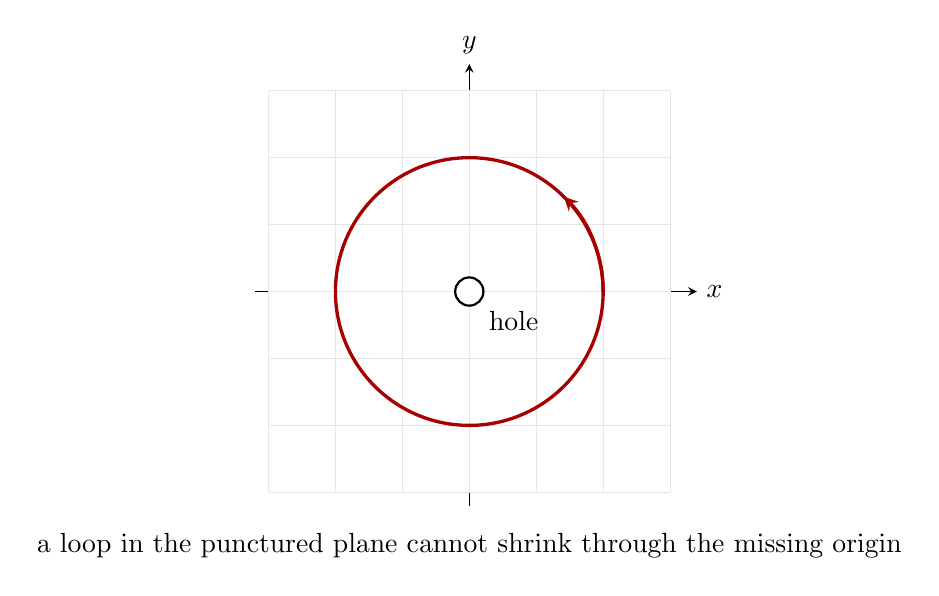
\begin{tikzpicture}[scale=0.85, >=stealth]
    \draw[->] (-3.2,0) -- (3.4,0) node[right] {\(x\)};
    \draw[->] (0,-3.2) -- (0,3.4) node[above] {\(y\)};

    \draw[gray!20, step=1] (-3,-3) grid (3,3);

    \draw[very thick, red!65!black] (0,0) circle (2);
    \draw[->, very thick, red!65!black] (2,0) arc[start angle=0,end angle=45,radius=2];

    \fill[white] (0,0) circle (6pt);
    \draw[thick] (0,0) circle (6pt);
    \node[below right] at (0.15,-0.15) {hole};

    \node at (0,-3.8) {a loop in the punctured plane cannot shrink through the missing origin};
\end{tikzpicture}
\caption{The form \(\alpha=\frac{-y\,dx+x\,dy}{x^2+y^2}\) has zero curl away from the
origin, but its integral around a loop enclosing the origin is \(2\pi\).}
\end{figure}

So what is going on?

Locally, \(\alpha\) really is a differential.  On the right half-plane \(x>0\), define
\[
    \theta=\arctan\left(\frac{y}{x}\right).
\]
Then
\[
    \theta_x=\frac{-y}{x^2+y^2},
    \qquad
    \theta_y=\frac{x}{x^2+y^2}.
\]
Therefore
\[
\boxed{
    d\theta=\alpha
}
\]
on the right half-plane.

The same thing works on many other smaller patches.  We can choose a continuous angle
function on a patch that does not wrap all the way around the origin.

But there is no single continuous angle function on the whole punctured plane.  After
one full counterclockwise trip around the origin, the angle has increased by
\[
    2\pi.
\]
It has not returned to its original value as an ordinary single-valued function should.

This is the difference between local and global.

\[
\boxed{
\begin{array}{c}
\text{Zero curl gives local potentials.}\\[1mm]
\text{A simply connected domain lets those local potentials glue into one global potential.}\\[1mm]
\text{A hole can prevent the gluing.}
\end{array}
}
\]

The scalar curl
\[
    Q_x-P_y
\]
is therefore a local measurement.  It detects tiny rotation.  It cannot, by itself, see a
missing point that a large loop winds around.  The next chapter supplies the missing
global bookkeeping: Green's theorem will add the local curl over a region and compare
it to circulation around the boundary.  That is where the hidden hole finally has to
show itself.
\section{Warning examples}
\label{sec:13.7}

Section \ref{sec:13.6} gave a useful test:
\[
    P_y=Q_x
\]
in the plane, or
\[
    \nabla\times\mathbf F=\mathbf 0
\]
in space.  But it also gave a warning: this test is local.  It checks tiny rotation near
each point.  It does not, by itself, know the shape of the whole domain.

This section collects the traps in one place.  They are worth seeing slowly, because most
mistakes with conservative fields come from forgetting one of them.

\subsection{Curl zero but no global potential on a punctured plane}

Consider the \(1\)-form
\[
    \alpha=\frac{-y\,dx+x\,dy}{x^2+y^2}
\]
on the punctured plane
\[
    D=\mathbb R^2\setminus\{(0,0)\}.
\]
The origin is missing, so the denominator is never zero on \(D\).

Write
\[
    \alpha=P\,dx+Q\,dy,
\]
where
\[
    P(x,y)=\frac{-y}{x^2+y^2},
    \qquad
    Q(x,y)=\frac{x}{x^2+y^2}.
\]
Compute:
\[
\begin{aligned}
P_y
&=
\frac{-(x^2+y^2)+2y^2}{(x^2+y^2)^2}\\
&=
\frac{y^2-x^2}{(x^2+y^2)^2},
\end{aligned}
\]
and
\[
\begin{aligned}
Q_x
&=
\frac{(x^2+y^2)-2x^2}{(x^2+y^2)^2}\\
&=
\frac{y^2-x^2}{(x^2+y^2)^2}.
\end{aligned}
\]
Thus
\[
    P_y=Q_x
\]
everywhere on \(D\).

So the local curl test passes.

Now integrate around the unit circle
\[
    C:\quad \mathbf r(t)=(\cos t,\sin t),
    \qquad 0\le t\le2\pi.
\]
Along this circle,
\[
    x=\cos t,\qquad y=\sin t,
\]
so
\[
    dx=-\sin t\,dt,
    \qquad
    dy=\cos t\,dt.
\]
Then
\[
\begin{aligned}
\alpha
&=
\frac{-(\sin t)(-\sin t\,dt)+(\cos t)(\cos t\,dt)}
{\cos^2t+\sin^2t}\\
&=
dt.
\end{aligned}
\]
Therefore
\[
\boxed{
    \oint_C \alpha=2\pi.
}
\]

If \(\alpha\) were exact on all of \(D\), then
\[
    \alpha=d\phi
\]
for some potential \(\phi\), and every closed-curve integral would be zero:
\[
    \oint_C d\phi=0.
\]
But this closed-curve integral is \(2\pi\).  So \(\alpha\) is not exact on the punctured
plane.

\begin{figure}[h]
\centering
\begin{tikzpicture}[scale=0.85, >=stealth]
    \draw[->] (-3.2,0) -- (3.4,0) node[right] {\(x\)};
    \draw[->] (0,-3.2) -- (0,3.4) node[above] {\(y\)};

    \draw[gray!20, step=1] (-3,-3) grid (3,3);

    \foreach \a in {0,30,...,330} {
        \pgfmathsetmacro{\x}{2*cos(\a)}
        \pgfmathsetmacro{\y}{2*sin(\a)}
        \draw[->, blue!65!black, thick]
            (\x,\y) -- ++({-0.35*sin(\a)},{0.35*cos(\a)});
    }

    \draw[very thick, red!65!black] (0,0) circle (2);
    \draw[->, very thick, red!65!black] (2,0) arc[start angle=0,end angle=45,radius=2];

    \fill[white] (0,0) circle (6pt);
    \draw[thick] (0,0) circle (6pt);
    \node[below right] at (0.15,-0.15) {missing};

    \node at (0,-4.0) {\(\alpha=\dfrac{-y\,dx+x\,dy}{x^2+y^2}\)};
\end{tikzpicture}
\caption{The form \(\alpha\) has zero curl away from the origin, but a loop around the
missing origin has integral \(2\pi\).}
\end{figure}

The moral is not that the curl test is wrong.  The moral is that the curl test is local.
A loop can detect a hole that no tiny derivative sees.

\subsection{A path-dependent integral with the same endpoints}

Path independence is a strong property.  It says that every path from \(A\) to \(B\)
gives the same integral.  Here is a simple field where that fails.

Let
\[
    \eta=-y\,dx+x\,dy.
\]
Move from
\[
    A=(0,0)
\]
to
\[
    B=(1,1).
\]

First take the straight path
\[
    C_1:\quad \mathbf r(t)=(t,t),
    \qquad 0\le t\le1.
\]
Then
\[
    x=t,\qquad y=t,\qquad dx=dt,\qquad dy=dt.
\]
So
\[
    \eta=-t\,dt+t\,dt=0.
\]
Therefore
\[
\boxed{
    \int_{C_1}\eta=0.
}
\]

Now take the broken path \(C_2\): first go east from \((0,0)\) to \((1,0)\), then go
north from \((1,0)\) to \((1,1)\).

On the eastward segment,
\[
    y=0,\qquad dy=0,
\]
so
\[
    -y\,dx+x\,dy=0.
\]
On the northward segment,
\[
    x=1,\qquad dx=0,
\]
so
\[
    -y\,dx+x\,dy=dy.
\]
Thus
\[
    \int_{C_2}\eta
    =
    \int_0^1 dy
    =
    1.
\]
So
\[
\boxed{
    \int_{C_2}\eta=1.
}
\]

The endpoints are the same, but the integrals are different:
\[
    \int_{C_1}\eta=0,
    \qquad
    \int_{C_2}\eta=1.
\]
So \(\eta\) is not exact, and its integral is not path independent.

The curl test sees the problem immediately:
\[
    P=-y,\qquad Q=x,
\]
so
\[
    Q_x-P_y=1-(-1)=2.
\]
This form carries rotation everywhere.

\begin{figure}[h]
\centering
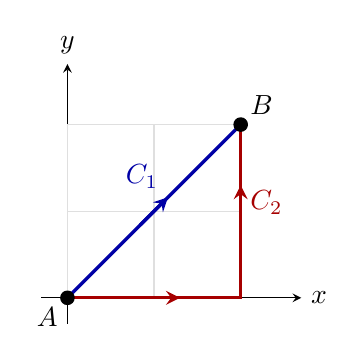
\begin{tikzpicture}[scale=2.2, >=stealth]
    \draw[->] (-0.15,0) -- (1.35,0) node[right] {\(x\)};
    \draw[->] (0,-0.15) -- (0,1.35) node[above] {\(y\)};

    \draw[gray!25, step=0.5] (0,0) grid (1,1);

    \coordinate (A) at (0,0);
    \coordinate (B) at (1,1);
    \coordinate (M) at (1,0);

    \draw[very thick, blue!65!black] (A) -- (B);
    \draw[->, very thick, blue!65!black] (0.42,0.42) -- (0.58,0.58);
    \node[blue!65!black, left] at (0.58,0.7) {\(C_1\)};

    \draw[very thick, red!65!black] (A) -- (M) -- (B);
    \draw[->, very thick, red!65!black] (0.35,0) -- (0.65,0);
    \draw[->, very thick, red!65!black] (1,0.35) -- (1,0.65);
    \node[red!65!black, right] at (1,0.55) {\(C_2\)};

    \fill (A) circle (1.2pt);
    \fill (B) circle (1.2pt);

    \node[below left] at (A) {\(A\)};
    \node[above right] at (B) {\(B\)};
\end{tikzpicture}
\caption{The same endpoints can give different work when the field is not conservative.}
\end{figure}

A conservative field has no memory of the route.  This one does.

\subsection{A vector field with a singularity hidden at the origin}

The most dangerous mistake is to compute a curl on the points where a field is defined
and then silently pretend the field is defined everywhere.

Return to
\[
    \mathbf A(x,y)=
    \left(
        \frac{-y}{x^2+y^2},
        \frac{x}{x^2+y^2}
    \right).
\]
This is the vector field associated with
\[
    \alpha=\frac{-y\,dx+x\,dy}{x^2+y^2}.
\]
It is not defined at the origin.

Around a circle of radius \(R>0\),
\[
    \mathbf r(t)=(R\cos t,R\sin t),
    \qquad 0\le t\le2\pi,
\]
we have
\[
    dx=-R\sin t\,dt,
    \qquad
    dy=R\cos t\,dt.
\]
The numerator becomes
\[
\begin{aligned}
-y\,dx+x\,dy
&=
-(R\sin t)(-R\sin t\,dt)+(R\cos t)(R\cos t\,dt)\\
&=
R^2\,dt.
\end{aligned}
\]
The denominator is
\[
    x^2+y^2=R^2.
\]
So
\[
    \alpha=dt,
\]
and therefore
\[
\boxed{
    \oint_{C_R}\alpha=2\pi
}
\]
for every radius \(R>0\).

This is strange at first.  The circle can be tiny:
\[
    R=10^{-6}.
\]
The circulation is still
\[
    2\pi.
\]

The reason is that the field gets stronger near the missing point.  Its length is
\[
    \|\mathbf A(x,y)\|
    =
    \frac{1}{\sqrt{x^2+y^2}}.
\]
On a circle of radius \(R\), the field has size \(1/R\).  The circumference is \(2\pi R\).
Their product stays roughly
\[
    \frac1R\cdot 2\pi R=2\pi.
\]

The origin is not a harmless missing point.  It is where the circulation is hiding.

So the statement
\[
    \nabla\times\mathbf A=\mathbf 0
\]
is true only on the punctured plane.  It is not a statement about the whole disk
containing the origin, because \(\mathbf A\) is not a vector field there.

\[
\boxed{
    \text{Before applying any theorem, check the domain of the field.}
}
\]

\subsection{Why the domain matters as much as the formula}

The same formula can behave differently on different domains.

Again take
\[
    \alpha=\frac{-y\,dx+x\,dy}{x^2+y^2}.
\]

On the right half-plane
\[
    D_+=\{(x,y):x>0\},
\]
define
\[
    \theta(x,y)=\arctan\left(\frac{y}{x}\right).
\]
Then
\[
    \theta_x=
    \frac{-y}{x^2+y^2},
    \qquad
    \theta_y=
    \frac{x}{x^2+y^2}.
\]
So
\[
\boxed{
    d\theta=\alpha
}
\]
on \(D_+\).  On the right half-plane, the form is exact.

But on the punctured plane
\[
    D=\mathbb R^2\setminus\{(0,0)\},
\]
the same formula is not exact, because
\[
    \oint_{\text{unit circle}}\alpha=2\pi.
\]

And on the whole plane
\[
    \mathbb R^2,
\]
the same formula does not even define a \(1\)-form, because it is undefined at
\((0,0)\).

\[
\begin{array}{c|c|c}
\text{Domain} & \text{Status of }\alpha & \text{Reason} \\ \hline
x>0 & \text{exact} & \alpha=d\arctan(y/x)\\[1mm]
\mathbb R^2\setminus\{(0,0)\} & \text{closed but not exact} &
\displaystyle \oint \alpha=2\pi\\[2mm]
\mathbb R^2 & \text{not defined} & \text{denominator is }0\text{ at the origin}
\end{array}
\]

This is why we never say only
\[
    \omega=P\,dx+Q\,dy.
\]
We say:
\[
    \omega=P\,dx+Q\,dy
    \quad\text{on a domain }D.
\]

The formula tells us the local measuring rule.  The domain tells us which paths are
allowed, which loops can shrink, and which singularities have been removed.  A
potential function is not just a formula.  It is a formula that works continuously and
single-valuedly on the whole domain.

These warnings look like exceptions, but they are really pointing toward a theorem.
The form
\[
    \alpha
\]
has no local curl away from the origin, yet a loop around the origin detects something
global.  To connect local curl with boundary circulation, we need a theorem that adds
curl over a whole region.  That theorem is Green's theorem.

\section{Chapter review and applications}
\label{sec:13.8}

Chapter \ref{ch:13} began with arrows attached to points and ended with a warning:
arrows are not enough.  The domain matters, orientation matters, and a line integral
can remember the path.

Here are the main tools in one place.

\subsection{Skills: line integrals and potentials}

There are two different kinds of line integrals in this chapter.

\[
\begin{array}{c|c|c|c}
\text{Integral} & \text{Notation} & \text{Uses} & \text{Direction matters?} \\ \hline
\text{scalar line integral}
&
\displaystyle \int_C f\,ds
&
\text{length, mass, average value}
&
\text{no}
\\[3mm]
\text{work integral / \(1\)-form integral}
&
\displaystyle \int_C P\,dx+Q\,dy+R\,dz
&
\text{work, circulation, potentials}
&
\text{yes}
\end{array}
\]

For a parametrized curve
\[
    \mathbf r(t)=(x(t),y(t),z(t)),
    \qquad a\le t\le b,
\]
the scalar line integral is
\[
\boxed{
    \int_C f\,ds
    =
    \int_a^b f(\mathbf r(t))\|\mathbf r'(t)\|\,dt.
}
\]
The speed
\[
    \|\mathbf r'(t)\|
\]
turns parameter time into arc length.

For a \(1\)-form
\[
    \omega=P\,dx+Q\,dy+R\,dz,
\]
the line integral is
\[
\boxed{
    \int_C \omega
    =
    \int_a^b
    \left[
        P(\mathbf r(t))x'(t)
        +
        Q(\mathbf r(t))y'(t)
        +
        R(\mathbf r(t))z'(t)
    \right]dt.
}
\]
Here
\[
    dx=x'(t)\,dt,\qquad dy=y'(t)\,dt,\qquad dz=z'(t)\,dt.
\]
No norm appears.  Orientation survives.

\[
\begin{array}{c|c}
\text{Question} & \text{Best tool} \\ \hline
\text{How long is the curve?} & \displaystyle \int_C 1\,ds\\[2mm]
\text{What is the mass of a wire?} & \displaystyle \int_C \rho\,ds\\[2mm]
\text{What work does a force field do?} & \displaystyle \int_C \mathbf F\cdot d\mathbf r\\[2mm]
\text{Is the integral only an endpoint difference?} & \text{look for a potential}\\[1mm]
\text{Is a plane form locally compatible with a potential?} & P_y=Q_x\\[1mm]
\text{Is a space field locally compatible with a potential?} & \nabla\times\mathbf F=\mathbf 0
\end{array}
\]

The exact case is the easiest case, once we recognize it.  If
\[
    \omega=d\phi,
\]
then
\[
\boxed{
    \int_C \omega=\phi(B)-\phi(A),
}
\]
where \(A\) is the starting point and \(B\) is the ending point.

This is the Fundamental Theorem of Calculus in curve form.

\subsubsection*{A final worked review problem}

Let
\[
    \omega=(2xy+z)\,dx+(x^2+3z)\,dy+(x+3y)\,dz.
\]
Find
\[
    \int_C \omega
\]
along any path from
\[
    A=(0,0,1)
\]
to
\[
    B=(2,1,3),
\]
if the integral is path independent.

First look for a potential \(\phi\).  If
\[
    \omega=d\phi,
\]
then
\[
    \phi_x=2xy+z.
\]
Integrate with respect to \(x\):
\[
    \phi=x^2y+xz+g(y,z).
\]
Now differentiate this with respect to \(y\):
\[
    \phi_y=x^2+g_y(y,z).
\]
We need
\[
    \phi_y=x^2+3z,
\]
so
\[
    g_y=3z.
\]
Thus
\[
    g(y,z)=3yz+h(z).
\]
Now
\[
    \phi=x^2y+xz+3yz+h(z).
\]
Differentiate with respect to \(z\):
\[
    \phi_z=x+3y+h'(z).
\]
We need
\[
    \phi_z=x+3y.
\]
So
\[
    h'(z)=0.
\]
One potential is
\[
\boxed{
    \phi(x,y,z)=x^2y+xz+3yz.
}
\]
Therefore
\[
\begin{aligned}
\int_C \omega
&=
\phi(B)-\phi(A)\\
&=
\phi(2,1,3)-\phi(0,0,1)\\
&=
(2^2\cdot1+2\cdot3+3\cdot1\cdot3)-0\\
&=
4+6+9\\
&=
19.
\end{aligned}
\]
So
\[
\boxed{
    \int_C \omega=19.
}
\]
No parametrization of \(C\) was needed.

\subsubsection*{The exterior derivative thread}

This chapter also prepared the next step in the differential-forms story.

A function is a \(0\)-form.  Its exterior derivative is
\[
    d\phi=\phi_x\,dx+\phi_y\,dy+\phi_z\,dz.
\]
This is the \(1\)-form version of the gradient.

For a plane \(1\)-form
\[
    \omega=P\,dx+Q\,dy,
\]
the exterior derivative is
\[
\boxed{
    d\omega=(Q_x-P_y)\,dx\wedge dy.
}
\]
The coefficient
\[
    Q_x-P_y
\]
is the scalar curl.

So the plane curl test
\[
    Q_x-P_y=0
\]
can be written as
\[
    d\omega=0.
\]
Exact forms satisfy
\[
    \omega=d\phi,
\]
and therefore
\[
    d\omega=d(d\phi)=0.
\]
This is the first concrete appearance of the rule
\[
\boxed{
    d^2=0.
}
\]

\subsection{Project: work done in a nonconservative field}

The field
\[
    \mathbf F(x,y)=(-y,x)
\]
is the simplest rotational field.  Its work form is
\[
    \eta=-y\,dx+x\,dy.
\]
It is not conservative, because
\[
    Q_x-P_y=1-(-1)=2.
\]
So a particle can return to where it started and still have nonzero total work done by
the field.

This project reveals a pattern that is too beautiful to be accidental.

\subsubsection*{A rectangle}

Let \(R\) be the rectangle
\[
    0\le x\le a,
    \qquad
    0\le y\le b.
\]
Orient its boundary counterclockwise.  That means the rectangle stays on your left as
you walk around it.

Compute
\[
    \oint_{\partial R} -y\,dx+x\,dy.
\]

There are four sides.

On the bottom side,
\[
    y=0,\qquad dy=0,
\]
so
\[
    -y\,dx+x\,dy=0.
\]

On the right side,
\[
    x=a,\qquad dx=0,\qquad 0\le y\le b,
\]
so
\[
    -y\,dx+x\,dy=a\,dy.
\]
The contribution is
\[
    \int_0^b a\,dy=ab.
\]

On the top side,
\[
    y=b,\qquad dy=0,
\]
and the path goes from \(x=a\) to \(x=0\).  The form becomes
\[
    -b\,dx.
\]
The contribution is
\[
    \int_a^0 -b\,dx=ab.
\]

On the left side,
\[
    x=0,\qquad dx=0,
\]
so
\[
    -y\,dx+x\,dy=0.
\]

Adding the four sides,
\[
\boxed{
    \oint_{\partial R} -y\,dx+x\,dy=2ab.
}
\]
But
\[
    ab=\operatorname{Area}(R).
\]
So
\[
\boxed{
    \oint_{\partial R} -y\,dx+x\,dy
    =
    2\,\operatorname{Area}(R).
}
\]

\begin{figure}[h]
\centering
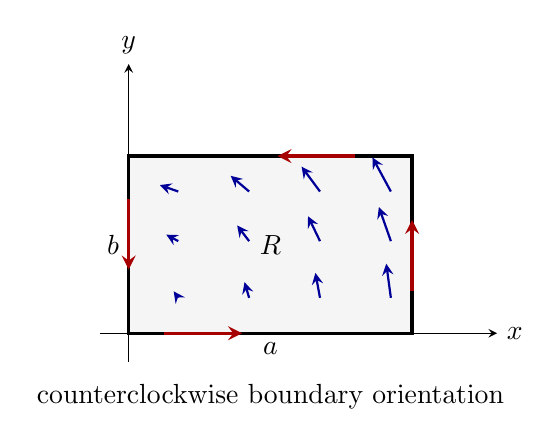
\begin{tikzpicture}[scale=0.9, >=stealth]
    \draw[->] (-0.4,0) -- (5.2,0) node[right] {\(x\)};
    \draw[->] (0,-0.4) -- (0,3.8) node[above] {\(y\)};

    \draw[fill=gray!8, very thick] (0,0) rectangle (4,2.5);

    \draw[->, very thick, red!65!black] (0.5,0) -- (1.6,0);
    \draw[->, very thick, red!65!black] (4,0.6) -- (4,1.6);
    \draw[->, very thick, red!65!black] (3.2,2.5) -- (2.1,2.5);
    \draw[->, very thick, red!65!black] (0,1.9) -- (0,0.9);

    \node[below] at (2,0) {\(a\)};
    \node[left] at (0,1.25) {\(b\)};
    \node at (2,1.25) {\(R\)};

    % Adjusted grid points and reduced scale to 0.13 to keep arrows inside
    \foreach \x in {0.7, 1.7, 2.7, 3.7} {
        \foreach \y in {0.5, 1.3, 2.0} {
            \draw[->, blue!60!black, thick]
                (\x,\y) -- ++({-0.13*\y},{0.13*\x});
        }
    }

    \node at (2,-0.9) {counterclockwise boundary orientation};
\end{tikzpicture}
\caption{The rotational field \((-y,x)\) does positive work around a positively oriented
rectangle.}
\end{figure}
The coefficient \(2\) is not a coincidence.  It is the scalar curl:
\[
    Q_x-P_y=2.
\]

So the rectangle calculation says
\[
\boxed{
    \oint_{\partial R}\eta
    =
    \iint_R 2\,dA.
}
\]
The left side is a boundary integral.  The right side is an area integral over the region.

\subsubsection*{A circle}

For a circle of radius \(R\), use
\[
    \mathbf r(t)=(R\cos t,R\sin t),
    \qquad 0\le t\le2\pi.
\]
Then
\[
    dx=-R\sin t\,dt,
    \qquad
    dy=R\cos t\,dt.
\]
So
\[
\begin{aligned}
-y\,dx+x\,dy
&=
-(R\sin t)(-R\sin t\,dt)
+
(R\cos t)(R\cos t\,dt)\\
&=
R^2\,dt.
\end{aligned}
\]
Thus
\[
\boxed{
    \oint_C -y\,dx+x\,dy
    =
    \int_0^{2\pi}R^2\,dt
    =
    2\pi R^2.
}
\]
But the area of the disk is
\[
    \pi R^2.
\]
Again,
\[
\boxed{
    \oint_C -y\,dx+x\,dy
    =
    2\,\operatorname{Area}(\text{disk}).
}
\]

\subsubsection*{A polygon and the shoelace formula}

Try the same integral around a polygon with vertices
\[
    (x_1,y_1),(x_2,y_2),\ldots,(x_n,y_n),
\]
listed counterclockwise, with
\[
    (x_{n+1},y_{n+1})=(x_1,y_1).
\]
On the straight edge from \((x_i,y_i)\) to \((x_{i+1},y_{i+1})\), a parametrization is
\[
    x(t)=x_i+t(x_{i+1}-x_i),
\]
\[
    y(t)=y_i+t(y_{i+1}-y_i),
    \qquad 0\le t\le1.
\]
Then
\[
    dx=(x_{i+1}-x_i)\,dt,
    \qquad
    dy=(y_{i+1}-y_i)\,dt.
\]
Substitution gives
\[
    -y\,dx+x\,dy
    =
    \bigl(x_i y_{i+1}-x_{i+1}y_i\bigr)\,dt.
\]
So the edge contribution is
\[
    x_i y_{i+1}-x_{i+1}y_i.
\]
Adding all edges,
\[
\boxed{
    \oint_{\partial P}-y\,dx+x\,dy
    =
    \sum_{i=1}^n
    \bigl(x_i y_{i+1}-x_{i+1}y_i\bigr).
}
\]
But the shoelace formula says
\[
\boxed{
    \operatorname{Area}(P)
    =
    \frac12
    \sum_{i=1}^n
    \bigl(x_i y_{i+1}-x_{i+1}y_i\bigr)
}
\]
for a counterclockwise polygon.  Therefore
\[
\boxed{
    \oint_{\partial P}-y\,dx+x\,dy
    =
    2\,\operatorname{Area}(P).
}
\]

The rotational field has become an area-measuring device.  By doing work only around
the boundary, it finds the area inside.

That is the surprise Green's theorem will explain.

\subsection{Hook: circulation becomes a two-dimensional integral}

The rectangle, circle, and polygon computations all point to the same hidden rule:
a boundary integral can equal an interior integral.

For
\[
    \eta=-y\,dx+x\,dy,
\]
we found
\[
    d\eta=2\,dx\wedge dy.
\]
The boundary integral measured
\[
    \oint_{\partial R}\eta,
\]
while the interior integral measured
\[
    \iint_R d\eta
    =
    \iint_R 2\,dx\wedge dy.
\]
For the shapes we computed,
\[
\boxed{
    \oint_{\partial R}\eta
    =
    \iint_R d\eta.
}
\]

The next chapter shows that this is not a trick of one special field.  For a large class of
regions \(R\) and \(1\)-forms
\[
    \omega=P\,dx+Q\,dy,
\]
Green's theorem says
\[
\boxed{
    \oint_{\partial R} \omega
    =
    \iint_R d\omega
    =
    \iint_R (Q_x-P_y)\,dx\wedge dy.
}
\]
The curl that was only a test in this chapter becomes something we can add over an
area.  A curve around the boundary will know what happened throughout the region
inside it.